\documentclass[12pt,twoside,leftblank]{../sty/mitthesis}
\usepackage{../sty/lgrind}
\usepackage{%
  xcolor,
  tikz,
  multirow,
  float,
  amssymb,
  amsmath,
  graphicx,
  fullpage,
  indentfirst,
  psfrag,
  mathrsfs,
  array,
  hyperref,
  color,
  arydshln,
  booktabs,
  empheq,
  mathtools,
  marginnote,
  fancyvrb,
  listings,
  mdframed,
  lipsum,
  listliketab,
  multicol,
  enumerate,
  lipsum,
  multirow,
  amsthm,
  thmtools,
  framed,
  verbatim,
  tabularx,
  pgfplots,
  enumitem
}
\usepackage[english]{babel}
\usepackage[compact]{titlesec}
\usepackage[titles]{tocloft}

\pagestyle{plain}
\usetikzlibrary{shapes,arrows,positioning,calc,matrix}

\newcommand{\figurepath}{../fig}

\usetikzlibrary{plotmarks}

\tikzstyle{squareblock}=[draw, fill=white!50, rectangle, minimum height=1cm, minimum width=1cm, inner sep= 2mm]
\tikzstyle{roundblock}=[draw, circle, fill=white!50, minimum height=1cm, inner sep= 1mm]
\tikzstyle{whitesum} = [draw, fill=white!40, circle, minimum width=0.6cm, inner sep= 1mm]
\tikzstyle{input} = [coordinate]
\tikzstyle{output} = [coordinate]
\tikzstyle{tee} = [coordinate]
\tikzstyle{block} = [draw, rectangle, minimum height=1cm, minimum width=2cm]
\tikzstyle{sum} = [draw, circle, node distance=1cm]
\tikzstyle{modelinput} = [coordinate]
\tikzstyle{modeloutput} = [coordinate]
\tikzstyle{regionoutput} = [coordinate]

\makeatletter
\pgfdeclareshape{satnode}{
\inheritsavedanchors[from={rectangle}]
\inheritbackgroundpath[from={rectangle}]
\inheritanchorborder[from={rectangle}]
\foreach\x in {center,north east,north west,north,south,south east,south west}{%
\inheritanchor[from={rectangle}]{\x}
}
\foregroundpath{%
\pgfpointdiff{\northeast}{\southwest}
\pgf@xa=\pgf@x\pgf@ya=\pgf@y%
\northeast%
\pgfpathmoveto{\pgfpoint{0}{0.45\pgf@ya}}
\pgfpathlineto{\pgfpoint{0}{-0.45\pgf@ya}}
\pgfpathmoveto{\pgfpoint{0.45\pgf@xa}{0}}
\pgfpathlineto{\pgfpoint{-0.45\pgf@xa}{0}}
\pgfpathmoveto{\pgfpointadd{\southwest}{\pgfpoint{-0.2\pgf@xa}{-0.3\pgf@ya}}}
\pgfpathlineto{\pgfpointadd{\southwest}{\pgfpoint{-0.5\pgf@xa}{-0.3\pgf@ya}}}
\pgfpathlineto{\pgfpointadd{\northeast}{\pgfpoint{-0.5\pgf@xa}{-0.3\pgf@ya}}}
\pgfpathlineto{\pgfpointadd{\northeast}{\pgfpoint{-0.4\pgf@xa}{-0.3\pgf@ya}}}
{%
   \pgftransformshift{\pgfpointadd{\northeast}{\pgfpoint{-0.4\pgf@xa}{-0.3\pgf@ya}}}
   \pgftransformscale{0.5}
   \pgfsetcolor{black}
   \pgftext[left]{}
}
\pgfusepath{stroke}
}
}
\makeatother

\pgfdeclarelayer{background}
\pgfdeclarelayer{foreground}
\pgfsetlayers{background,main,foreground}

\renewcommand{\theenumi}{\Alph{enumi}}

\begin{document}
\title{Adaptive Control of a Generic Hypersonic Vehicle}
\author{Daniel Philip Wiese}
\prevdegrees{B.S. University of California, Davis (2011)}
\department{Department of Mechanical Engineering}
\degree{Master of Science}
\degreemonth{June}
\degreeyear{2013}
\thesisdate{May 10, 2013}
\supervisor{Anuradha M. Annaswamy}{Senior Research Scientist}
\chairman{David E. Hardt}{Chairman, Department Committee on Graduate Students}
\maketitle

\cleardoublepage%
\setcounter{savepage}{\thepage}
\begin{abstractpage}
This thesis presents a an adaptive augmented, gain-scheduled baseline LQR-PI controller applied to the Road Runner six-degree-of-freedom generic hypersonic vehicle model.
Uncertainty in control effectiveness, longitudinal center of gravity location, and aerodynamic coefficients are introduced in the model, as well as sensor bias and noise, and input time delays.
The performance of the baseline controller is compared to the same design augmented with one of two different model-reference adaptive controllers: a classical open-loop reference model design, and modified closed-loop reference model design.
Both adaptive controllers show improved command tracking and stability over the baseline controller when subject to these uncertainties.
The closed-loop reference model controller offers the best performance, tolerating a reduced control effectiveness of 50\%, rearward center of gravity shift of -0.9 to -1.6 feet (6--11\% of vehicle length), aerodynamic coefficient uncertainty scaled $4\times$ the nominal value, and sensor bias of $+1.6$ degrees on sideslip angle measurement.
The closed-loop reference model adaptive controller maintains at least 73\% of the delay margin provided by the robust baseline design, tolerating input time delays of between 18--46 ms during 3 degree angle of attack doublet, and 80 degree roll step commands.

\end{abstractpage}

\cleardoublepage%

\section*{Acknowledgments}

I would like to thank my advisor Dr.\ Anuradha Annaswamy for her guidance during this research.
I would also like to thank Dr.\ Jonathan Muse and Dr.\ Michael Bolender in the Aerospace Systems Directorate at the Air Force Research Laboratory for providing the vehicle model for this research, giving their support and advice along the way, and providing direction during my summer work at AFRL.\@
Thanks to Dr.\ Eugene Lavretsky of Boeing Research \& Technology for contributing his invaluable advice and suggestions throughout this project.
Thanks also to all of my lab mates for our discussions and help through various research problems, and making lab enjoyable.
Their assistance and friendship over the last two years has been great.
I also want to thank Dr.\ Lutz, without whom I would not be where I am today.
I want to thank her for all of the encouragement and inspiration over the past five years, and for being a truly outstanding mentor.
Thanks as well to Bob for providing advice and wisdom.
I would like to thank all of my friends for their patience and understanding.
Finally, I would like to thank my Mom, Dad, and all of my family for their love and support all these years.

This research is funded by the Air Force Research Laboratory/Aerospace Systems Directorate grant FA 8650--07--2--3744 for the Michigan/AFRL Collaborative Center in Control Sciences, with Dr.\ Michael Bolender as technical monitor.

\pagestyle{plain}
\input{chapters/contents}
\chapter{Introduction}

\section{Background}

With a history spanning well over a half century, hypersonic flight continues to be a topic of significant research interest\ \cite{parker.control.2007,gibson.adaptive.2009,kothari.reusable.2010,dalle.envelope.2011,brocanelli.unstartrecovery.2012}.
Air-breathing hypersonic vehicles are particularly attractive due to their potential to serve as high speed passenger transports and long range weapon delivery systems, and provide cost-effective access to space.
Hypersonic vehicles are likely to be inherently unstable\ \cite{mcruer.hypersonic.1991,mirmirani.airbreathing.2005,bolender.hypersonicmodel.2007} and the integration of the airframe and engine in an air-breathing hypersonic vehicle contributes to additional modeling and control challenges.
With limited wind tunnel data, harsh and uncertain operating environments, poorly known physical models, and largely varying operating conditions, it is of great importance to ensure that any control scheme will be significantly robust to ensure safe operation during flight.

Unlike the transition from subsonic to supersonic flow, the physics of hypersonic flow do not differ from that of supersonic flow.
Instead, the distinction of hypersonic flow is made to stress the importance of certain physical phenomena which exist in all supersonic flows that become dominant at hypersonic speeds, typically defined to be flow at a Mach number of 5 or greater\ \cite{anderson.aerodynamics.2010}.
It wasn't until 1946, well into the study of such flow regimes, that this term was finally coined\ \cite{Tsien2012443}.
The high flight Mach numbers experienced by a hypersonic vehicle result in significant aerodynamic heating.
This aerodynamic heating can have a great impact on the material properties of the vehicle.
In addition to this coupling of aerodynamic and structural effects, the engines of air-breathing hypersonic vehicles are tightly integrated into the airframe of the vehicle, where long fore and aft sections of the vehicle make up large portions of the engine inlet and nozzle, respectively.
This tightly couples the engine dynamics with the airframe and structural dynamics as well as the aerodynamics\ \cite{chavez.flightdynamics.1994}.
The physics of hypersonic flow and these resulting interactions between all the components of the vehicle make the control of hypersonic vehicles very challenging.

A major challenge associated with the control of hypersonic vehicles, in addition to the interactions between airframe, engine, and structural dynamics, is the limited ability to accurately determine the aerodynamics characteristics\ \cite{maughmer.prediction.1989,schmidt.dynamics.1991,chavez.analytical.1994,coleman.hypersonic.2009}.
With the presence of such tight coupling between all aspects of a hypersonic vehicle, the ability to collect wind tunnel and flight data to study these interactions would be highly useful.
However, these tests are very difficult to do, and so much of the knowledge about a hypersonic vehicle's aerodynamics must come from physics-based models.
This makes accurate determination of the aerodynamic characteristics very difficult, making the design of a controller more difficult as well.

Another control challenge associated specifically with air breathing hypersonic vehicles is that of engine unstart.
Unstart is a phenomenon caused by several factors including thermal choking and insufficient air recovery at the inlet.
This ultimately leads to the upstream propagation of the shock train out of the inlet, effectively preventing air from entering the engine due to a standing normal shock in front of the isolator entrance\ \cite{curran.scramjet.2000}.
This causes an abrupt change in the pitching moment, an increase in drag, decrease in lift, loss of thrust, and potentially changes in vehicle yawing and rolling moments as well\ \cite{bolender.unstart.2009}.
If the flight path is such that it requires the GHV to unstart, the control law must be such that it can accommodate these large and sudden changes, thus ensuring stable flight can be maintained through unstart.

With all of the complex interactions between the different aircraft components, and high level of uncertainty in the models, the control of a hypersonic vehicle is very challenging.
These challenges have led to many advances in the design of flight control.

\section{History}

The science of aerodynamics was first invented in the early 1900s by Ludwig Prandtl in Germany.
The field of aerodynamics matured considerably over the next half-century, and during World War II, the Germans were beginning to approach hypersonic speeds in laboratory wind  tunnel tests at Mach 4.4, and with weapons such as the V-2 rocket approaching similar speeds\ \cite{heppenheimer.heatbarrier.2009}.
The hypersonic technology of the United States was substantially behind that of the Germans at the time, until the war ended and Wernher von Braun and his team of rocket scientists came to the United States.
Just over eleven years after the end of World War II, history was made when the X-2 became the fastest airplane ever, reaching a speed of almost Mach 3.2.
Moments after the record was broken, the plane lost control and began tumbling downwards toward Earth, destroying the plane and killing the pilot due to a mechanism known as inertial coupling\ \cite{nelson.flightcontrol.1998}.
This disaster made the consequences of not maintaining stability during high speed flight very real.

The study of hypersonics in the 1950s was also being propelled by the United States' interest in intercontinental ballistic missiles, which began with the X-17 rocket.
The accurate guidance of such missiles over long ranges was of particular importance, but it was the challenges associated with significant aerodynamic heating upon atmospheric re-entry that dominated research in this area during this time.
The first test of the X-17 took place in 1956 to investigate the re-entry of a hemispherical nose-cone, and reached a speed of Mach 12.4.
This research provided valuable information used in the Mercury program, which succeeded in putting the first American in space in 1961.
The inherently stable design of the Mercury capsule allowed safe atmospheric re-entry even without an effective control system.
While guidance, navigation and control (GNC) challenges of later hypersonic re-entry vehicles were more difficult, the effective control of atmospheric hypersonic vehicles such as the X-2 was a major problem that needed to be solved.

Following the testing of the X-2, the X-planes program continued in the late 1950s, with much of the knowledge gained through research to be used in the development of high performance fighter aircraft of the time.
One of the most notable hypersonic airplanes to ever fly, the X-15 pictured in Figure~\ref{fig:x15flying}, made its first flight in 1959.
The designers of the X-15 overcame many of the challenges associated with hypersonic flight.
The X-15 had to be very heat resistant to withstand the temperatures encountered during flight at nearly Mach 7, and the engine needed the power to propel the plane to these high speeds.
The flight envelope of the X-15 was so broad that reaction controls were used in addition to the aerodynamic control surfaces, which lost effectiveness above 100,000 feet altitude.
Transitioning between these two control systems was difficult as well.
In addition to these challenges, and more, the only significant source of aerodynamic data used in the development of the X-15 came from a single small hypersonic wind tunnel, making modeling for control especially challenging.
Despite these challenges, three variants of the X-15 made a combined total of nearly 200 flights over the next ten years following its first flight.
The third variant of the X-15, was the only of the three craft to include an adaptive controller as part of its stability augmentation system.
This adaptive controller attempted to adjust feedback gains to provide optimum angular rates as commanded by the pilot, and also provided a means to transition from aerodynamic to reaction controls, allowing the command of both control systems from a single control stick in the cockpit.
While the X-15 allowed hours of valuable flight data to be obtained, engineers were once again reminded of the consequences of faulty designs when the MH-96 adaptive controller aboard the X-15 failed to reduce the feedback gains upon re-entry, setting up a violent pitch oscillation which destroyed the aircraft and killed the pilot.

 \begin{figure}[h]
  \begin{center}
    \includegraphics[width=3.5in]{\figurepath/x15flying.jpg}
    \caption{North American X-15\label{fig:x15flying}}
  \end{center}
\end{figure}

Toward the end of the X-15's career, there was a building interest in a new, advanced air-breathing propulsion system for hypersonic flight, as opposed to the rocket propulsion used on the X-15 and its predecessors.
This Hypersonic Research Engine (HRE) was to utilize concepts first disclosed by The Johns Hopkins Universities' Applied Physics Lab in 1959, as part of a project known as Supersonic Combustion Ramjet Missle (SCRAM).
The scramjet engines were initialy designed as pods, much like conventional turbofans on commercial and transport aircraft.
Early plans called for a podded scramjet to be fitted on the X-15, but it was quickly realized that this would not be possible.
To make scramjets practical for use in flight, the engine would have to be integrated intimately in the airframe, using the fore and aft sections of the vehicle as part of the inlet and nozzle of the scramjet.
Development of scramjet technology was pushed forward in the early 1980s in part by the U.S. Air Force, in order to develop a single-stage-to-orbit vehicle to deliver military weapons systems to space.
This ultimately led to the National Aero-Space Plane (NASP) program, and the design of the 160 foot long Rockwell X-30.
This program lasted over ten years and lead to many advances in scramjet propulsion research and the study of flexible hypersonic vehicles, but no X-30 were ever built.

\begin{figure}[h]
  \begin{center}
    \includegraphics[width=3.5in]{\figurepath/nasa_x43.jpg}
    \caption{NASA X-43A}
  \end{center}
\end{figure}

Hypersonic research slowed for some years, until scramjet research emerged again in the early 1990s as part of a collaboration between the United States and Russia.
This collaboration saw scramjets mounted aboard rockets being tested in flight.
Control again became a critical challenge in hypersonic flight, this time in the control of the engines.
Fuel delivery had to be controlled precisely to keep the engines operating in supersonic combustion mode, and avoid a condition known as unstart.
Control systems aboard these rocket-mounted scramjets were designed to monitor pressures within the engines and adjust fuel flow to prevent unstart, but the early control systems were not yet ready for this demanding challenges.
An all-American effort at practical scramjet powered hypersonic flight was born in 1996 under the name Hyper-X\ \cite{freeman.hyperx.1997}.
Hyper-X was an eight year NASA program with the goal of demonstrating the viability of air-breathing hypersonic flight.
The demonstrator vehicle for this program, the X-43, was 12 feet long, and 5 feet wide.
The first flight took place in June 2001 and failed, but in March 2004 the X-43A became the first vehicle to ever be propelled during hypersonic flight by an air-breathing engine, reaching a speed of Mach 6.8 for 11 seconds.
The third flight in November 2004 lasted 10 seconds and reached a speed of Mach 9.6.
These ground breaking flights demonstrated the practicability of a scramjet powered hypersonic vehicle, and are alongside the X-15 in terms of importance in the history of hypersonic flight.

In the 1990s and 2000s, many hypersonics programs have been introduced, including HyTECH, HyShot, HyCause, HIFiRE, and more.
The most notable platform since the X-43A was the X-51, built by Boeing and managed by the U.S. Air Force Research Lab (AFRL).
While the X-43A demonstrated the feasibility of scramjet powered flight, a new record was set by the X-51 in 2010 by maintaining scramjet powered flight at 5 for 140 seconds.
The second X-51 flight took place in 2011 and ended early due to unstart, and during the third test flight the X-51 lost control and fell into the ocean.
History was made once again in May 2013, when the X-51 made the longest air-breathing hypersonic flight, maintaining Mach 5.1 for 240 seconds under its own power.

\begin{figure}[h]
  \begin{center}
    \includegraphics[width=3.5in]{\figurepath/boeing_x51_v3.jpg}
    \caption{Boeing X-51 waverider}
  \end{center}
\end{figure}

The history of hypersonic flight is still in the making, with current research centered around the sustained flight of air-breathing vehicles.
The previous trajectories flown by aircraft such as the X-15, X-43 and X-51 were fairly benign in that abrupt and sudden maneuvers were generally avoided, and the goal was to demonstrate primarily the ability of these experimental aircraft to maintain hypersonic flight under their own power.
As technology grows the demands of these vehicles will grow too.
Current research is being performed to develop new materials and engine designs for these vehicles, as well as advanced control systems which will allow complex maneuvers to be performed while maintaining stability even in situations where unstart conditions are encountered.


\section{Control Design}

Some of the challenges associated with the control of hypersonic vehicles throughout history has been discussed above.
These challenges include the limited wind tunnel data available to determine accurate models for control design, large flight envelopes with significant uncertainty in the operating environment, and need to cope with engine unstart, in addition to problems such as actuator failure, flexibility effects, and time delays.
This section discusses some of the existing methods developed to control hypersonic vehicles, and why the adaptive control structure used in this thesis was chosen.

The equations of motion which describe an aircraft are nonlinear, but in most cases it is acceptable to linearize these equations to facilitate control design and analysis.
This lead to the description of aircraft dynamics using the transfer function, and to simple stability augmentation systems such as roll and yaw dampers\ \cite{cook.flightdynamics.2007}.
These flight control systems were simple, low-order, linear dynamic feedback compensators such as lead-lag and PID, and typically used small feedback gains\ \cite{dazzo.linearcontrol.2003,mclean.flightcontrol.1990,yechout.flightmechanics.2003}.
Thorough frequency domain analysis was critical to ensure a robust design.
Optimal control techniques slowly began seeing use in flight control in the early 1980s with limited success, but have now become more widely used\ \cite{chandler.lqrshortcomings.1983,abzug.stability.2005,stevenslewis.aircraftcontrol.2003,stengel.flightdynamics.2004}.
Many robust, nonlinear, and adaptive control solutions are proposed in recent literature\ \cite{xu.adaptive.2004,gibson.adaptive.2008,hughes.hinfinity.2010,huang.robust.2012,bolender.hifire6.2012,rollins.nonlinear.2013} which include sliding mode, H2/H$_{\infty}$, dynamic inversion, and neural network control, as well as many other techniques.

\subsection{Need for Adaptive Control}

Adaptive control research was driven in the 1950s by the need for aircraft autopilots for aircraft that operated in a wide flight envelope, across which the aircraft dynamics change significantly\ \cite{astrom.feedback.1987}.
While many of the techniques described above offer their own unique advantages in certain applications, adaptive control is a particularly attractive candidate for dealing with the problems associated with the control of aircraft including hypersonic vehicles.
In order design any controller for a given dynamical system, a model is needed, and with any model there is uncertainty.

Aircraft dynamics can be reasonably approximated by a linearization about a trim flight condition.
The parametric uncertainties which are prevalent in aerospace applications such as control surface ineffectiveness, unknown aerodynamic coefficients, center of gravity shift, and more manifest themselves themselves in a way which is conducive to the design of an adaptive controller.
That is, many of the uncertainties associated with hypersonic vehicles can be represented as parametric ones, entering the system through the control channels.
An adaptive controller can contend easily with these and ensure the desired closed-loop performance is attained, when degradation of a robust baseline controller is inevitable.
The adaptive control structure taken in this thesis is then built around this linearized design model with the parametric uncertainties.
The controller is then applied to the evaluation model, and the efficacy of the controller is examined through simulation studies.

\section{Overview}

Chapter 2 introduces the dynamical equations describing the hypersonic vehicle model.
The assumptions used in this model are stated.
The equations of motion are linearized about a nominal flight condition, and the flight modes are analyzed.
The uncertainties which will be considered, and their representation in the linear model are presented.

Chapter 3 presents the linear baseline control structure which takes advantage of the decoupling of the various flight modes to design three independent control subsystems using state feedback control.
Each of the linear controllers is analyzed in the frequency domain to ensure good selection of the feedback gains for fast and robust performance.
The process of gain-scheduling this baseline controller across the flight envelope using dynamic pressure is explained.
The classical open-loop reference model (ORM), and modified closed-loop reference model (CRM) adaptive control architectures are presented.

Chapter 4 described uncertainties which the model will be subject to within the simulation environment.
Simulation results demonstrating the efficacy of the gain-scheduled baseline and adaptive-augmented baseline controller when the system is subject to various uncertainties are provided.

Chapter 5 provides the conclusions of this research, and describes a simple unstart model which may be used for future research regarding the adaptive control of air-breathing hypersonic vehicles.

\chapter{Hypersonic Vehicle Model}

The Generic Hypersonic Vehicle which is used as a platform for analysis and control design is shown in Figure~\ref{fig.ghvclouds}.
The Road Runner GHV is a small, pilotless, blended wing-body vehicle, with 3-D inlet and nozzle, and axisymmetric through-flow scramjet engine.
There are four aerodynamic control surfaces which can be moved independently, consisting of two elevons and two rudders.
The relevant vehicle properties are listed in Table~\ref{tab:vehicle_properties}.

\begin{figure}[h]
  \begin{center}
    \includegraphics[width=4.5in]{\figurepath/ghvmodelview.png}
    \caption{AFRL Road Runner generic hypersonic vehicle\ \cite{ruttle.ghv.2012}\label{fig.ghvclouds}}
  \end{center}
\end{figure}

The Road Runner GHV was developed by AFRL in an effort to create a publicly releasable hypersonic vehicle model for studies of operability, controllability, and aero-propulsion integration as described in Reference\ \cite{ruttle.ghv.2012}.
The objective was to design a common vehicle which would be relevant to the technical efforts of current hypersonic projects, including the HIFiRE 6 vehicle, which the Road Runner closely resembles, as can be seen in Reference\ \cite{bolender.hifire6.2012}.
This GHV was designed be launched on rocket to accelerate it to cruise at Mach 6, at a dynamic pressure of between 1000--2000 psf.
The mission profile for the GHV then required maneuvers to be performed during the middle of the cruise phase before descending and decelerating, and making an unpowered maneuver to evaluate the potential to make a controlled landing.
The GHV should have the capability to perform sustained maneuvers up to a load factor of up to approximately 2G.

\begin{table}[H]
  \centering
  \caption{Vehicle properties}
  \begin{tabular}{llr}
    \toprule
    Parameter & Unit & Value \\
    \midrule
    Gross weight & [lbm] & $1220.3$ \\
    Empty weight & [lbm] & $993.3$ \\
    Vehicle length & [in] & $175.9$ \\
    Span & [in] & $58.6$ \\
    Nose diameter & [in] & $11.0$ \\
    Tail diameter & [in] & $18.8$ \\
    \bottomrule
  \end{tabular}\label{tab:vehicle_properties}
\end{table}

The aerodynamic data for the Road Runner was calculated using Hypersonic Engineering Aerothermodynamic Trajectory Tool Kit (HEAT-TK), developed for the Air Force by Boeing\ \cite{carter.heattk.2005}, and the engine data is calculated using the Ramjet Performance Analysis (RJPA) code, developed at Johns Hopkins University's Applied Physics Lab.

\section{Modeling the GHV}

The equations of motion describing many aircraft can be derived assuming a flat, non-rotating Earth.
Due to the high flight speed of a hypersonic vehicle in the atmosphere, the rotation and curvature of the Earth are typically significant, and should not be neglected.
Thus, the governing equations of motion for the GHV are derived assuming the vehicle is a rigid body flying through the atmosphere of a spherical, rotating Earth.
The equations of motion describing the GHV are given in References\ \cite{etkin.atmosphericflight.1972,billamoria.eom.1995}, and will be presented here for completeness.

\subsubsection*{Notation}

In deriving and applying the equations of motion which govern the motion of an aircraft, care must be taken to carefully book-keep the various vector quantities which describe the position, velocity and orientation of the aircraft.
For instance, when considering the velocity of an aircraft, it must be kept clear both with which frame the velocity is with respect to, and in which frame the velocity vector is described.
Some of the standard notation describing the expression of vectors in various reference frames is outlined below.
\begin{itemize}
  \item{$f_{a}$ denotes reference frame $a$.}
  \item{$O_{a}$ denotes the origin of reference frame $a$.}
  \item{$V^{a}_{b}$ describes the velocity of the origin of reference frame $b$ relative to the axes of reference frame $a$, described using the coordinate system of reference frame $b$.}
  \item{$\omega^{a,b}_{c}$ describes the angular velocity of reference frame $a$ relative to reference frame $b$ described using the axes of reference frame $c$. Omission of the second superscript implies the angular velocity of coordinate system $a$ is with respect to inertial axes. When the subscript is omitted, it is implied this quantity is described in the coordinates of frame $a$. For example $\omega^{B}$ is the inertial angular velocity of frame $f_{B}$, described using the axes of frame $f_{B}$.}
  \item{The transformation $R_{ab}$ describes a vector transformation from being expressed in reference frame $b$ to being expressed in reference frame $a$.}
  \item{$\frac{dV_{a}}{dt}\bigr|_{b}$ denotes the rate of change of $V_{a}$ with respect to frame $b$.}
  \item{All vectors are describing a relation of frame $a$ to frame $b$ are described along the axes of frame $a$.}
\end{itemize}

In many cases, the equations of motion can be greatly simplified when studying the dynamics of an aircraft.
Such simplifications often center around assuming the Earth is flat, but this may be an oversimplification for problems of hypersonic atmospheric flight.
While this simplification still might be acceptable for calculations involving the attitude dynamics where the rotating earth terms are typically very small, in trajectory calculations the rotating earth terms for a hypersonic vehicle become non-negligible.
This section presents the equations of motion that describe the GHV.\@

\subsection{Equations of Motion}

The equations of motion are developed using an Earth-centered, Earth-frame $f_{EC}$ with origin at the center of a spherical, rotating Earth.
It is assumed that the atmosphere travels uniformly with Earth as it rotates with angular velocity $\omega_{\text{earth}}$ in inertial space, and that the aircraft is sufficiently rigid that flexible structural effects can be neglected.
The position of the GHV around Earth and relative to $f_{EC}$ is described by its latitude $\lambda$, longitude $\tau$, and distance from the center of the Earth, $\mathscr{R}$.
These three coordinates give the location of the vehicle-carried frame $f_{V}$, defined with $z$-axis always pointing toward the origin of $f_{EC}$.

\begin{figure}[h]
  \begin{center}
    \small
    \psfrag{N}[bc][bc]{$N$}
    \psfrag{wE}[bl][bl]{$\omega_{\text{earth}}$}
    \psfrag{xE}[bc][bc]{$x_{E}$}
    \psfrag{yE}[bc][bc]{$y_{E}$}
    \psfrag{FE}[bc][bc]{$f_{E}$}
    \psfrag{OE}[bc][bc]{$O_{E}$}
    \psfrag{zEC}[bc][bc]{$z_{I}$}
    \psfrag{zE}[bc][bc]{$z_{E}$}
    \psfrag{yEC}[bc][bc]{$y_{I}$}
    \psfrag{FEC}[bc][bc]{$f_{I}$}
    \psfrag{OEC}[bc][bc]{$O_{I}$}
    \psfrag{xEC}[bc][bc]{$x_{I}$}
    \psfrag{lambda}[bl][bl]{$\lambda$}
    \psfrag{tau}[bc][bc]{$\tau$}
    \psfrag{eq}[bl][bl]{Equator}
    \psfrag{mer}[br][br]{Meridian}
    \psfrag{xv}[br][br]{$x_{V}$}
    \psfrag{yv}[bl][bl]{$y_{V}$}
    \psfrag{zv}[tr][tr]{$z_{V}$}
    \psfrag{ov}[tl][tl]{$O_{V}$}
    \includegraphics[height=3.5in]{\figurepath/earth_fig_4.eps}
    \caption{Reference frames\label{globe_fig}}
  \end{center}
\end{figure}

The vehicle carrying frame $f_{V}$ is a frame with origin attached to vehicle at the CG, and the z-axis $O_{V}z_{V}$ is defined to point vertically downward along the local $g$ vector.
$O_{V}x_{V}$ is defined to point north, and $O_{V}y_{V}$ east as shown in Figure~\ref{globe_fig}.
The vehicle-carried frame has angular velocity $\omega^{V}$ due to the curvature of the earth.
The body-fixed reference frame $f_{B}$ is a right-handed coordinate system attached to the GHV with $x$-axis pointing towards the nose of the aircraft along the longitudinal axis, and the $z$-axis pointing down.
This body-fixed axis system is used to derive the equations of motion for the GHV.\@

In deriving the equations of motion, the only additional assumption is that the centripetal acceleration due to $\omega_{\text{earth}}$ is negligible.
The equations of motion describe the dynamics of the GHV around the Earth when subject to external forces and moments.
These forces and moments, given in the body axes by $F_{B}$, and $M_{B}$ respectively, are due to the thrust and aerodynamic forces acting on the GHV, and are taken from pre-determined look-up tables within the simulation.
The aerodynamic forces depend on on control surface deflection angle, dynamic pressure, angle of attack, and sideslip angle.
The thrust forces depend on on control surface deflection angle, dynamic pressure, and angle of attack.

\subsubsection*{Force Equations}

The force equation describing the the motion of the GHV center of gravity in body axes is given as the following
\begin{equation}
  \label{eqn:forceeqn}
  \frac{dV^{A}_{B}}{dt}\biggr|_{B}+\omega^{B}\times V^{A}_{B}+
  \omega^{E}_{B}\times V^{A}_{B}+\omega^{E}_{B}\times(\omega^{E}_{B}\times\mathscr{R})=
  g+(F_{A}+F_{T})/m
\end{equation}
where $V^{A}_{B}$ denotes the velocity of $f_{B}$ relative to the atmosphere-fixed reference frame, and $\omega^{E}_{B}$ is the inertial angular velocity of the Earth-fixed frame $f_{E}$, described using the coordinate system of the body reference frame.
Note in this work that the atmosphere is assumed fixed with respect to the earth, so $f_{A}=f_{E}$.
The components of the atmospheric velocity are
\begin{equation}
  V_{B}^{A}=
  \bigr[
  \begin{array}{ccc}
    u & v & w
  \end{array}\bigr]^{\top}
\end{equation}
The force vector $F_{B}$ that represents all non-gravitational forces acting on the body in body axes is given by
\begin{equation}
  F_{B}=
  \bigr[
  \begin{array}{ccc}
    X & Y & Z
  \end{array}\bigr]^{\top}
\end{equation}
In the Equation (\ref{eqn:forceeqn}) this force is separated into aerodynamic and propulsive contributions as $F_{B}=F_{A}+F_{T}$ where the aerodynamic and propulsive forces have components given by
\begin{equation}
  \begin{split}
    F_{A}&=
    \bigr[
    \begin{array}{ccc}
      X_{A} & Y_{A} & Z_{A}
    \end{array}\bigr]^{\top} \\
    F_{T}&=
    \bigr[
    \begin{array}{ccc}
      X_{T} & Y_{T} & Z_{T}
    \end{array}\bigr]^{\top}
  \end{split}
\end{equation}

\subsubsection*{Moment equations}

The vehicle moments are described by the following equation.
Note the absence of any rotor contributions to the vehicle moment, as the scramjet engine lacks moving parts, unlike jet-turbine powered craft.
\begin{equation}
  \label{eqn:momenteqn}
  J\frac{d\omega^{B}}{dt}\biggr|_{B}+\omega^{B}\times J\omega^{B}=M_{A}+M_{T}
\end{equation}
$\omega_{B}$ is the angular velocity of the body frame relative to the inertial frame, with the rate of change evaluated in the body frame, and components
\begin{equation}
  \omega^{B}=
  \bigr[
  \begin{array}{ccc}
    p & q & r
  \end{array}\bigr]^{\top}
\end{equation}
The total torque in body axes is given by
\begin{equation}
  M_{B}=
  \bigr[
  \begin{array}{ccc}
    L & M & N
  \end{array}\bigr]^{\top}
\end{equation}
This total moment is split into the contributions due to aerodynamic and propulsive moments in Equation (\ref{eqn:momenteqn}) as $M_{B}=M_{A}+M_{T}$ where the aerodynamic and propulsive moments have components given by
\begin{equation}
  \begin{split}
    M_{A}&=
    \bigr[
    \begin{array}{ccc}
      L_{A} & M_{A} & N_{A}
    \end{array}\bigr]^{\top} \\
    M_{T}&=
    \bigr[
    \begin{array}{ccc}
      L_{T} & M_{T} & N_{T}
    \end{array}\bigr]^{\top}
  \end{split}
\end{equation}
The moment of inertia matrix $J$ is given by
\begin{equation}
  J=
  \begin{bmatrix}
    J_{xx} & -J_{xy} & -J_{xz} \\
    -J_{xy} & J_{yy} & -J_{yz} \\
    -J_{xz} & -J_{yz} & J_{zz}
  \end{bmatrix}
\end{equation}
Without any simplification, expansion of the moment equations would become very cumbersome.
In general, aircraft are symmetric about the $x-z$ plane, mass is uniformly distributed, and the body coordinate system is oriented such that $J_{xy}=J_{yz}=0$.
This allows the moment of inertia matrix for the GHV to be simplified to
\begin{equation}
  J=
  \begin{bmatrix}
    J_{xx} & 0 & -J_{xz} \\
    0 & J_{yy} & 0 \\
    -J_{xz} & 0 & J_{zz}
  \end{bmatrix}
\end{equation}

\subsubsection*{Orientation Equations}

The orientation, or kinematic equations describe the orientation of the aircraft body axes with respect to the vehicle carried frame.
The relationship between Euler rates and body angular velocities in the vehicle- carried frame is given by

\begin{equation}
  \label{eulr_ss_eqn}
  \left[
  \begin{array}{c}
    \dot{\phi} \\
    \dot{\theta} \\
    \dot{\psi}
  \end{array}\right]=
  \left[
  \begin{array}{ccc}
    1 & \tan(\theta)\sin(\phi) & \tan(\theta)\cos(\phi) \\
    0 & \cos(\phi) & -\sin(\phi) \\
    0 & \sin(\phi)/\cos(\theta) & \cos(\phi)/\cos(\theta)
  \end{array}\right]
  \left[
  \begin{array}{c}
    p_{v} \\
    q_{v} \\
    r_{v}
  \end{array}\right]
\end{equation}
where $\phi$, $\theta$, and $\psi$ are the roll, pitch, and yaw or heading angles, respectively, and are known as the Euer angles.
The components of angular velocities $p_{v}$, $q_{v}$, and $r_{v}$ are for the aircraft with body-fixed reference frame $f_{B}$ and are relative to the vehicle-carrying frame $f_{V}$.
These components of angular velocity are about the $x$, $y$, and $z$ body axes, respectively.
The relative angular velocities of the GHV are related to the vehicle absolute angular velocities by
\begin{equation}
  \begin{bmatrix}
    p_{v} \\
    q_{v} \\
    r_{v}
  \end{bmatrix}=
  \begin{bmatrix}
    p \\
    q \\
    r
  \end{bmatrix}-R_{BV}
  \begin{bmatrix}
    (\omega_{\text{earth}}+\dot{\tau})\cos{\lambda} \\
    -\dot{\lambda} \\
    -(\omega_{\text{earth}}+\dot{\tau})\sin{\lambda}
  \end{bmatrix}
\end{equation}
where $R_{BV}$ is the orthogonal rotation matrix given by
\begin{equation}
  R_{BV}=
  \begin{bmatrix}
    \cos{\theta}\cos{\psi} & \cos{\theta}\sin{\psi} & -\sin{\theta} \\
    \sin{\phi}\sin{\theta}\cos{\psi}-\cos{\phi}\sin{\psi} & \sin{\phi}\sin{\theta}\sin{\psi}+\cos{\phi}\cos{\psi} & \sin{\phi}\cos{\theta}\\
    \cos{\phi}\sin{\theta}\cos{\psi}+\sin{\phi}\sin{\psi} & \cos{\phi}\sin{\theta}\sin{\psi}-\sin{\phi}\cos{\psi} & \cos{\phi}\cos{\theta}
  \end{bmatrix}
\end{equation}

The reason for the distinction between relative and absolute angular rates in the above equations is due to the spherical Earth.
If a hypersonic vehicle was flying continuous circles around the world, the Euler rate's would all be zero as the aircraft would be stationary relative to the vehicle carried frame.
However, the absolute angular rates would be non-zero, as the vehicle carried frame would be rotating as it moved over the surface of the Earth.

\subsubsection*{Navigation Equations}

The location, or navigation equations describe the location of the origin of the body fixed coordinate system with respect to the inertial axes.
The quantities describing this location are latitude, longitude, and altitude.
The navigation kinematic equation is given by
\begin{equation}
  \begin{bmatrix}
    \dot{\lambda}\mathscr{R} \\
    \dot{\tau}\mathscr{R}\cos{\lambda} \\
    -\dot{\mathscr{R}}
  \end{bmatrix}=R_{VB}
  \begin{bmatrix}
    u \\
    v \\
    w
  \end{bmatrix}
\end{equation}
where $R_{VB}=R_{BV}^{-1}$.

\subsubsection*{Construction of Equations}

These equations were assembled in a \textsc{Simulink} model with main component blocks as indicated in Figure~\ref{fig.ghvblocks}.
The forces and moments are calculated from aerodynamic and engine data stored in look-up tables.

\begin{figure}[H]
  \begin{center}
    \includegraphics[width=6.0in]{\figurepath/block_eqns_2.eps}
    \caption{Equation of motion model blocks\ \cite{etkin.atmosphericflight.1972}\label{fig.ghvblocks}}
  \end{center}
\end{figure}

\section{State Space Representation}

The equations of motion can be represented in state-space form as
\begin{equation}
  \dot{X}=f({X},U)
\end{equation}
with state vector
\begin{equation}
  \label{eqn:fullstatevectorx}
  X=\left[
  \begin{array}{cccccccccccc}
    V_{T} &  \alpha & q &\theta & h & \beta &p & r & \phi &\psi &\lambda & \tau
  \end{array}\right]^{\top}
\end{equation}
where $V_{T}$ is the total velocity, $\alpha$ and $\beta$ are the angle of attack and sideslip angle, $\phi$, $\theta$, and $\psi$ are the roll, pitch, and yaw angles, $p$, $q$, and $r$ are the absolute angular velocity components, and $\lambda$, $\tau$, and $h$ are the latitude, longitude, and altitude, of the GHV, respectively.
The input vector is given by
\begin{equation}
  \label{eqn:fullcontrolvector}
  U=\left[
  \begin{array}{cccc}
    u_{\text{th}} & u_{\text{elv}} & u_{\text{ail}} & u_{\text{rud}}
  \end{array}\right]^{\top}
\end{equation}
where $u_{\text{th}}$, $u_{\text{elv}}$, $u_{\text{ail}}$, and $u_{\text{rud}}$ are the throttle, elevator, aileron, and throttle inputs, respectively.
The entries of the state vector are arranged so as to facilitate separation of the lateral and longitudinal equations of motion during control design.
The deflection of the elevons are accomplished through static mixing, combining differential and collective deflections from the aileron and elevator commands, respectively, while both rudders are actuated together using the single rudder input.
The control vector $U_{5}$ contains the deflections of the right and left elevons ($u_{r,\text{elv}}$, $u_{l,\text{elv}}$), rudders ($u_{r,\text{rud}}$, $u_{l,\text{rud}}$), and throttle as
\begin{equation}
  U_{5}=
  \bigr[
  \begin{array}{ccccc}
    u_{\text{th}} & u_{r,\text{elv}} & u_{l,\text{elv}} & u_{r,\text{rud}}  & u_{l,\text{rud}}
  \end{array}\bigr]^{\top}
\end{equation}
The control allocation matrix $M$ is the matrix which defines the following transformation between control vectors $U_{5}$ and $U$ as
\begin{equation}
  U=MU_{5}
\end{equation}
where control allocation matrix is
\begin{equation}
  M=
  \left[
  \begin{array}{ccccc}
    1 & 0 & 0 & 0 & 0 \\
    0 & 1/2 & 1/2 & 0 & 0 \\
    0 & 1/2 & -1/2 & 0 & 0 \\
    0 & 0 & 0 & 1/2 & 1/2 \\
  \end{array}\right]
\end{equation}

\subsection{Actuator and Sensor Models}

\paragraph{Throttle} The propulsion system is modeled as a first order system with a cutoff frequency of 10 rad/s, with transfer function
\begin{equation*}
  G_{\text{th}}(s)=\frac{\omega_{\text{th}}}{s+{\omega_{\text{th}}}}
\end{equation*}
While the physics of the engine happen on time scales order of magnitude faster than the rest of the dynamics, this simple model was proposed to capture fuel system delivery limits.

\paragraph{Control Surfaces} Second order actuators with rate and deflection limits were included in the simulation model on all four of the aerodynamic control surfaces.
The transfer function for the control surface actuators is
\begin{equation}
  G_{\text{cs}}(s)=\frac{{\omega_{n}}^{2}}{s^{2}+2\zeta\omega_{n}s+{\omega_{n}}^{2}}
\end{equation}
and the block diagram for the control surfaces as implemented is shown in Figure~\ref{fig:actuator_block} where the signal $u_{\text{cmd}}$ is generated by the controller, and due to the actuator dynamics the actual control surface deflection is given by $u_{\text{sat}}$.

\begin{figure}[H]
  \begin{center}
    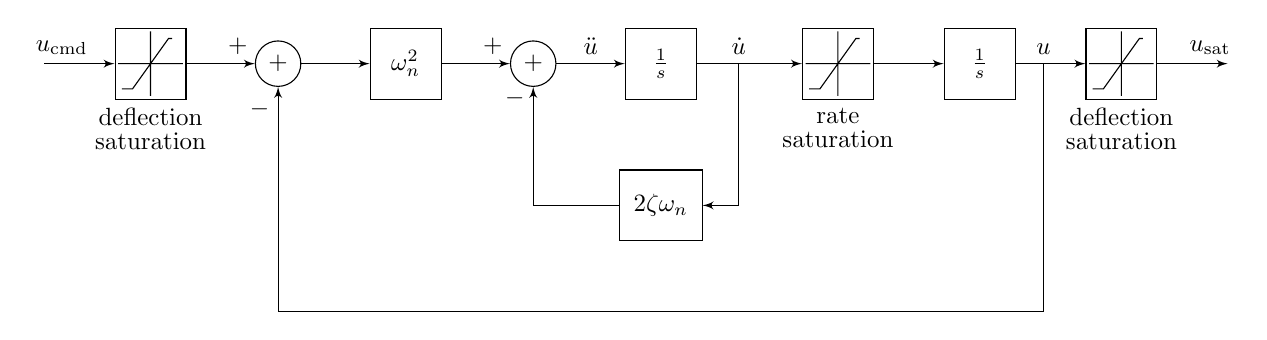
\begin{tikzpicture}[auto, scale=0.9, every node/.style={transform shape}, node distance=1.5cm, >=latex']
    \node[input](input1){};
    \node[satnode,draw,fill=white, minimum height=1.0cm, minimum width=1.0cm, right of=input1, node distance=1.5cm, label=below:{\shortstack{deflection \\ saturation}}] (block1){};
    \node[whitesum, right of=block1,node distance=1.8cm](sum1){$+$};
    \node[squareblock, right of=sum1,node distance=1.8cm] (block2){$\omega_{n}^{2}$};
    \node[whitesum, right of=block2, node distance=1.8cm](sum2){$+$};
    \node[squareblock, right of=sum2,node distance=1.8cm] (block3){$\frac{1}{s}$};
    \node[satnode,draw,fill=white, minimum height=1.0cm, minimum width=1.0cm, right of=block3, node distance=2.5cm, label=below:{\shortstack{rate \\ saturation}}] (block4){};
    \node[squareblock, right of=block4,node distance=2.0cm] (block5){$\frac{1}{s}$};
    \node[satnode,draw,fill=white, minimum height=1.0cm, minimum width=1.0cm, right of=block5, node distance=2.0cm, label=below:{\shortstack{deflection \\ saturation}}] (block6){};
    \node[output, right of=block6,node distance=1.5cm] (output1) {};
    \node[squareblock, below of=block3,node distance=2.0cm] (block7){$2\zeta\omega_{n}$};
    \node[tee,below of=block7,node distance=1.5cm] (tee1){};
    %Draw lines
    \draw[->](input1) -- node[near start]{$u_{\text{cmd}}$} (block1);
    \draw[->](block1) -- node[near end]{$+$} (sum1);
    \draw[->](sum1) -- (block2);
    \draw[->](block2) -- node[near end]{$+$} (sum2);
    \draw[->](sum2) -- node{$\ddot{u}$} (block3);
    \draw[->](block3) -- node[pos=0.4,name=u]{$\dot{u}$} (block4);
    \draw[->](block4) -- (block5);
    \draw[->](block5) -- node[pos=0.4,name=y]{$u$} (block6);
    \draw[->](block6) -- node[near end]{$u_{\text{sat}}$} (output1);
    \draw[->](u) |- (block7);
    \draw[->](block7) -| node[pos=0.95]{$-$} (sum2);
    \draw[-](y) |- (tee1);
    \draw[->](tee1) -| node[pos=0.95]{$-$} (sum1);
    \end{tikzpicture}
    \caption{Second order actuator block diagram\label{fig:actuator_block}}
  \end{center}
\end{figure}

The relevant values used in the second order aerodynamic control surface actuator model are listed in Table~\ref{tab:actuator}.
\begin{table}[H]
  \centering
  \caption{Second order aerodynamic control surface actuator parameters\label{tab:actuator}}
  \begin{tabular}{llc}
    \toprule
    Parameter & Unit & Value \\
    \midrule
    Elevon deflection limit & [deg] & $-30$ to $30$ \\
    Rudder deflection limit & [deg] & $-30$ to $30$ \\
    Elevon rate limit & [deg/s] & $-100$ to $100$ \\
    Tail rate limit & [deg/s] & $-100 $ to $100$ \\
    Damping ratio $\zeta$ & & $0.7$ \\
    Natural frequency $\omega_{n}$ & [rad/s] & $150$ \\
    \bottomrule
  \end{tabular}
\end{table}

\paragraph{Sensor Filters} First order low-pass filters were placed at the sensor outputs in order to model the effects of a navigation filter in the loop, and reduce sensor noise being fed back to the controller.
The velocity filter has a cutoff frequency of 20 rad/s, while the incidence, angular rate, and Euler angle sensor filters all have a cutoff frequency of 150 rad/s.

\subsection{Implementation}

The GHV simulation block diagram is in Figure~\ref{fig:ghvcontrolblock}.
The controller was implemented in discrete time and operated at 100 Hz with a zero-order hold on the control signal output.
The output sensors are operated at 600 Hz also using zero-order hold samping, white noise was injected into the sensor signals, and a variable input time delay was used.

\begin{figure}[H]
  \begin{center}
    \begin{tikzpicture}[auto, scale=0.8, every node/.style={transform shape}, node distance=1.0cm, >=latex']
    \node[squareblock, minimum height=1cm, minimum width=2cm, label=below:{100 Hz}] (block1){Controller};
    \node[input,left=of block1.170, node distance=2.0cm] (j1) {};
    \node[left of=j1, node distance=0.5cm] (input1) {};
    \node[input,left=of block1.190, node distance=1.0cm] (input2) {};
    \node[squareblock, minimum width=1cm, right of=block1, node distance=2.5cm] (block2) {$\tau_{\text{delay}}$};
    \node[squareblock, minimum height=1cm, minimum width=1.0cm, label=below:{\shortstack[c]{Actuator\\Dynamics}}, right of=block2,node distance=2.5cm, inner sep= 1mm] (block3) {\includegraphics[width=1.6cm]{\figurepath/actuator_image.png}};
    \node [right of=block3,draw=black, anchor=west,node distance=2.0cm, minimum width=2cm, label=below:{Plant}, inner sep= 0mm] (block4) {\includegraphics[width=4cm]{\figurepath/ghvclouds.pdf}};
    \node[whitesum, right of=block4,node distance=3.0cm] (sum1) {$+$};
    \node[input, above of=sum1,node distance=1.2cm](input3){};
    \node[squareblock, minimum width=1cm, right of=sum1, node distance=2.0cm] (block5) {ZOH};
    \node[squareblock, minimum width=1cm, right of=block5, node distance=2.0cm] (block6) {Filter};
    \node[output, right of=block6,node distance=2.0cm] (output1) {};
    \node[tee, below of=block3,node distance=1.8cm](tee1){};
    %Draw lines
    \draw[-](input1) -- node[near start]{$z_{\text{cmd}}$} (j1);
    \draw[->](j1) -- (block1.170);
    \draw[->](input2) -- (block1.190);
    \draw[->](block1) -- (block2);
    \draw[->](block2) -- (block3);
    \draw[->](block3) -- (block4);
    \draw[->](block4) -- (sum1);
    \draw[->](input3) -- (sum1);
    \draw[->](sum1) -- (block5);
    \draw[->](block5) -- node[name=n,pos=0.5]{}(block6);
    \draw[->](block6) -- node[name=y,pos=0.7]{} node[near end]{$x$}(output1);
    \draw[-](y) |- node[pos=0.9] {} (tee1);
    \draw[-](tee1) -| (input2);
    %Model box
    \begin{pgfonlayer}{background}
      \path (block5 |- block5)+(-1.0,0.7) node (c) {};
      \path (block6 -| block6)+(1.0,-0.7) node (d) {};
      \path[fill=gray!20, draw, dashed] (c) rectangle (d);
    \end{pgfonlayer}
    \node [above of=sum1, node distance = 1.5cm] {noise};
    \node[below of=n,node distance=1.2cm]{600 Hz};
    \end{tikzpicture}
    \caption{GHV flight control simulation block diagram\label{fig:ghvcontrolblock}}
  \end{center}
\end{figure}

The discretization of the controller and sensor models as well as the addition of time delay, actuator dynamics, and noise makes the evaluation model a more realistic representation of the actual hardware on which the proposed control laws would be implemented.
This is to better evaluate through simulations the robustness capability of the control design as it contends with these realistic effects.

\section{Open-Loop Analysis}

The open-loop behavior of the GHV was analyzed about a nominal flight condition of $M=6$, $h=80,000$ ft, corresponding to a dynamic pressure of 1474 psf.
The geographical coordinates and heading of the GHV are insignificant in the equations of motion for the purposes of inner-loop control law development, and these state variables are dropped from the state vector (\ref{eqn:fullstatevectorx}) for trim, linearization, and control.
\begin{equation}
  \label{eqn:truncstatevectorx}
  X=\bigr[
  \begin{array}{ccccccccc}
    V_{T} &  \alpha & q &\theta & h & \beta &p & r & \phi
  \end{array}\bigr]^{\top}
\end{equation}
The state $X$ from this point forward is used to mean the truncated state (\ref{eqn:truncstatevectorx}), as it contains the primary quantities describing the vehicle dynamics that are to be controlled.
The navigation components of (\ref{eqn:fullstatevectorx}) will evolve as a consequence of controlling (\ref{eqn:truncstatevectorx}) and in practice would be commanded through an outer-loop guidance controller.
The dynamics of the system with truncated state are described by
\begin{equation}
  \label{eqn:xdotfxu}
  \dot{X}=f({X},U)
\end{equation}
The equilibrium, or trim state $X_{\text{eq}}$ and input $U_{\text{eq}}$ satisfy
\begin{equation}
  \label{eqn:eqptdef}
  \dot{X}_{\text{eq}}=f({X}_{\text{eq}},U_{\text{eq}})=0
\end{equation}
The equilibrium state and input are found for the nominal steady, level cruise condition, and Equation (\ref{eqn:xdotfxu}) is linearized about this trim condition as follows.
Defining $x$ and $u$ to be state and input perturbations about equilibrium, the state and input can be expressed as
\begin{equation}
  \begin{split}
    X&=X_{\text{eq}}+x \\
    U&=U_{\text{eq}}+u
  \end{split}
\end{equation}
Differentiating (\ref{eqn:xdotfxu})
\begin{equation}
  \begin{split}
    \dot{X}=\dot{x}&=f(X, U) \\
    &=f(X_{\text{eq}}+x,U_{\text{eq}}+u)
  \end{split}
\end{equation}
Performing a Taylor series expansion, neglecting second order terms and higher
\begin{equation*}
  \dot{x}= f(X_{\text{eq}},U_{\text{eq}})+\left.\frac{\partial f(X,U)}{\partial X}\right|_{\text{eq}}x+\left.\frac{\partial f(X,U)}{\partial U}\right|_{\text{eq}}u+\epsilon
\end{equation*}
where the subscript $(\cdot)_{\text{eq}}$ indicates these quantities be evaluated at the equilibrium point.
With $f(X_{\text{eq}},U_{\text{eq}})=0$, the linearization results in the state-space system given by
\begin{equation}
  \label{eqn:linss}
  \dot{x}=Ax+Bu
\end{equation}
where
\begin{equation}
  A=\left.\frac{\partial f(X,U)}{\partial X}\right|_{\text{eq}}^{}
  \hspace{0.5in}
  B=\left.\frac{\partial f(X,U)}{\partial U}\right|_{\text{eq}}^{}
\end{equation}
Using this linear system, the open-loop dynamic modes of the GHV during the nominal steady level cruise condition are analyzed through a sensitivity analysis.
It is also important to note that the perturbation state $x$ of the linear system in Equation (\ref{eqn:linss}) will be represented as having the following components.
\begin{equation}
  x=\bigr[
  \begin{array}{ccccccccc}
    \Delta V_{T} & \Delta\alpha & \Delta q & \Delta\theta & \Delta h & \Delta\beta & \Delta p & \Delta r & \Delta\phi
  \end{array}\bigr]^{\top}
\end{equation}
The perturbation input for the linear system is equivalently defined as
\begin{equation}
  u=\left[
  \begin{array}{cccc}
    \Delta\delta_{\text{th}} & \Delta\delta_{\text{elv}} & \Delta\delta_{\text{ail}} & \Delta\delta_{\text{rud}}
  \end{array}\right]^{\top}
\end{equation}
In following sections, this notation is abused by not explicitly including the $\Delta$ preceding each component to indicate that the components of the state vector $x$ and input vector $u$ are in fact perturbation states and inputs, respectively.
This is done only when there is no possibility of confusion, and so when referring to the state and control input of the linear system given by Equation (\ref{eqn:linss}) the following notation will be used
\begin{equation}
  \label{eqn:perturbedstatevectorx}
  x=\bigr[
  \begin{array}{ccccccccc}
    V_{T} & \alpha & q &\theta & h & \beta &p & r & \phi
  \end{array}\bigr]^{\top}
\end{equation}
\begin{equation}
  u=\left[
  \begin{array}{cccc}
    \delta_{\text{th}} & \delta_{\text{elv}} & \delta_{\text{ail}} & \delta_{\text{rud}}
  \end{array}\right]^{\top}
\end{equation}

\subsection{Modal Analysis}

Given a linear system such as Equation (\ref{eqn:linss}) it is often of interest to examine the system modes.
Conventional aircraft usually have modes which are quite predictable in their characteristics from one vehicle to the next, but with an aircraft such as the GHV, the significant state variables in the different modes may differ from those of conventional aircraft.
Because of this it is crucial to analyze the system modes to better understand the dynamics of the GHV, and to facilitate the control design process.

The sensitivity matrix for the linear system given in Equation (\ref{eqn:linss}) is calculated, which contains the desired modal information.
The sensitivity analysis aims to determine which entries in a given eigenvector are small when the units of each state variable are not the same.
This method examines slight changes in the initial condition of each state separately in order to determine whether this change will influence some modes more strongly than others.
This analysis will provide knowledge of what modes the GHV exhibits, which states are dominant in each of these modes, as well as the stability of these modes.

\subsubsection*{Mode Sensitivity}
Consider the linear system (\ref{eqn:linss}) describing the GHV dynamics, with perturbation state vector given by (\ref{eqn:perturbedstatevectorx}).
This section outlines the method presented in\ \cite{etkin.atmosphericflight.1972} of applying a linear transformation to a state space system to obtain a system represented in characteristic coordinate system to facilitate the modal analysis and calculation of the sensitivity matrix.
Considering only the initial condition response, the following autonomous system results
\begin{equation}
  \label{eqn:xdotax}
  \dot{x}=Ax
\end{equation}
The following nonsingular transformation is introduced
\begin{equation}
  x=\mathbb{V}q
\end{equation}
where $\mathbb{V}\triangleq[\begin{array}{ccc} \mathrm{v}_{1} & \cdots & \mathrm{v}_{n} \end{array}]$ is the modal matrix made up of the eigenvectors or $A$ as shown.
Note that this transformation will not alter the eigenvalues or eigenvectors of the system in (\ref{eqn:xdotax}).
Using this transformation
\begin{equation}
  \dot{q}=\tilde{A}q
\end{equation}
where
\begin{equation}
  \tilde{A}=\mathbb{V}^{-1}A\mathbb{V}
\end{equation}
The matrix $\mathbb{V}^{-1}A\mathbb{V}$ can be expressed as
\begin{equation}
  A\mathbb{V}
  =A \left[
  \begin{array}{ccc}
    \mathrm{v}_{1} & \cdots & \mathrm{v}_{n}
  \end{array} \right]
  =\left[
  \begin{array}{ccc}
    A\mathrm{v}_{1} & \cdots & A\mathrm{v}_{n}
  \end{array}\right]
  =\left[
  \begin{array}{ccc}
    \mathrm{v}_{1}\lambda_{1} & \cdots & \mathrm{v}_{n}\lambda_{n}
  \end{array}\right]
  =\mathbb{V}\Lambda%
\end{equation}
giving
\begin{equation}
  \dot{q}=\Lambda{q}
\end{equation}
where $\Lambda$ is the diagonal matrix of eigenvalues.
The solution is given by
\begin{equation}
  q(t)=e^{\Lambda{t}}q(0)
\end{equation}
The unforced response of the system in response to initial conditions is of interest.
In particular, an initial condition is selected as a scalar multiple of an eigenvector $\mathrm{v}_{i}$
\begin{equation}
  x(0)=\alpha_{i}\mathrm{v}_{i}
\end{equation}
Using the linear transformation
\begin{equation}
  q(0)=\mathbb{V}^{-1}x(0)=\alpha_{i}\mathbb{V}^{-1}\mathrm{v}_{i}
\end{equation}
Since $\mathbb{V}^{-1}\mathbb{V}=\mathbb{I}$ where $\mathbb{I}$ is the identity matrix, $\mathbb{V}^{-1}\mathrm{v}_{i}$ is just the $\mathrm{i^{th}}$ column of $\mathbb{I}$.
In other words, the initial condition $q(0)$ corresponding to the selected $x(0)$ will be a column vector of zeros, with the exception of the entry $\alpha_{i}$ in the $\mathrm{i^{th}}$ row.
The response of the state $x(t)$ from this initial condition is given by
\begin{equation}
  \begin{split}
    x(t)&=\mathbb{V}e^{\Lambda{t}}\alpha_{i}\mathbb{V}^{-1}\mathrm{v}_{i} \\
    &=\alpha_{i}\mathbb{V}e^{\Lambda{t}}
    \bigr[
    \begin{array}{ccccc}
      0 & \hdots & 1 & \hdots & 0
    \end{array}\bigr]^{\top}
  \end{split}
\end{equation}
Expanding
\begin{equation}
  \begin{split}
    x(t)&=\alpha_{i}
    \left[
    \begin{array}{ccc}
      \mathrm{v}_{1} & \cdots & \mathrm{v}_{n}
    \end{array} \right]
    \left[
    \begin{array}{cccc}
      e^{\lambda_{1}t} & 0 & \cdots & 0 \\
      0 & e^{\lambda_{2}t} & \cdots & 0 \\
      \vdots & \vdots & \ddots & \vdots \\
      0 & 0 & \cdots & e^{\lambda_{n}t}
    \end{array}\right]
    \begin{bmatrix}
      0 \\
      \vdots \\
      1 \\
      \vdots \\
      0
    \end{bmatrix} \\
    &=\alpha_{i}e^{\lambda_{i}t}\mathrm{v}_{i}
  \end{split}
\end{equation}
This shows that only the mode corresponding to $\lambda_{i}$ will be present in the response from an initial condition along the $\mathrm{i^{th}}$ eigenvector.
The general response in terms of $x$ is given by summing the individual responses starting from each eigenvector initial condition
\begin{equation*}
  x(t)=\sum \limits_{i=1}^{n} \alpha_{i}e^{\lambda_{i}t}\mathrm{v}_{i}
\end{equation*}
Based on this unforced modal response, if any entries in $\mathrm{v}_{i}$ are small relative to the others, the corresponding states are thus not influential in determining the initial condition response.

\subsubsection*{Calculating the Sensitivity Matrix}

In this section the methods of\ \cite{manual.durham.2002} used to calculate the sensitivity matrix for $\tilde{A}$ are outlined.
The matrix $\mathbb{V}$ and its inverse $\mathbb{V}^{-1}$ are first calculated.
The rows of $\mathbb{V}$ are denoted using $r_{i}$, and the columns of $\mathbb{V}^{-1}$ as $c_{i}$
\begin{equation*}
  \mathbb{V}=
  \bigr[
  \begin{array}{cccc}
    r_{1}^{\top} & r_{2}^{\top} & \hdots & r_{n} ^{\top}
  \end{array}\bigr]^{\top}
  \hspace{0.5in}
  \mathbb{V}^{-1}=\left[
  \begin{array}{cccc}
    c_{1} & c_{2} & \cdots & c_{n}
  \end{array}\right]
\end{equation*}
The diagonal matrices $C_{i}$ are formed using the elements of $c_{i}$
\begin{equation*}
  c_{i}=\left[
  \begin{array}{c}
    c_{i,1} \\
    c_{i,2} \\
    \vdots \\
    c_{i,n}
  \end{array}\right] \hspace{0.5in}
  C_{i}=\left[
  \begin{array}{cccc}
  c_{i,1} & 0 & \cdots & 0 \\
  0 & c_{i,2} & \cdots & 0 \\
  \vdots & \vdots & \ddots & \vdots \\
  0 & 0 & \cdots & c_{i,n}
  \end{array}\right]
\end{equation*}
The $n \times n$ sensitivity matrix $S$ is defined as
\begin{equation*}
  S\equiv\left[
  \begin{array}{c}
    r_{1}C_{1} \\
    r_{2}C_{2} \\
    \vdots \\
    r_{n}C_{n}
  \end{array}\right]
\end{equation*}

\subsubsection*{Sensitivity Matrix Analysis: Nominal Flight Condition}
The sensitivity matrix $S$ is shown in Table~\ref{sensmat_fc1_1} for a nominal flight condition of flight Mach number $M=6$ and altitude $h=80,000$ ft, giving a dynamic pressure of $\bar{q}=1,474$ psf.

\begin{table}[H]
  \centering
  \caption{Sensitivity matrix: nominal flight condition}
  \fontsize{8pt}{8pt}\selectfont
  \begin{tabularx}{0.95\textwidth}{|X|XXXXX|XXXX|} %{|c|ccccc|cccc|} chktex 44
    \cline{2-10}
    \multicolumn{1}{c|}{} & $\lambda_{1}$ & $\lambda_{2}$ & $\lambda_{3}$ & $\lambda_{4}$ & $\lambda_{5}$ & $\lambda_{6}$ & $\lambda_{7}$ & $\lambda_{8}$ & $\lambda_{9}$ \\
    \multicolumn{1}{c|}{} &  -2.24 & -4.87 & 1.89 & \multicolumn{2}{c|}{$1.37\pm 0.76\mathrm{j}$} & \multicolumn{2}{c}{$0\pm 0.12\mathrm{j}$} & -0.0039 & -0.0272 \\
    \hline % chktex 44
    $V_{T}$ & 3.44E-05 & 1.22E-13 & 6.57E-05 & 1.34E-10 & 1.34E-10 & 0.0022 & 0.0022 & \textbf{0.9955} & 2.46E-09 \\
    \hline % chktex 44
    $\alpha$ & \textbf{0.3618} & 7.31E-10 & \textbf{0.3226} & 3.04E-08 & 3.04E-08 & \textbf{0.1578} & \textbf{0.1578} & 3.04E-05 & 4.96E-10 \\
    $q$     & \textbf{0.4823} & 1.05E-09 & \textbf{0.5103} & 4.97E-08 & 4.97E-08 & 0.0036 & 0.0036 & 2.48E-07 & 4.57E-12 \\
    $\theta$ & 0.0088 & 1.79E-11 & 0.0160 & 3.92E-09 & 3.92E-09 & \textbf{0.4876} & \textbf{0.4876} & 5.32E-05 & 1.59E-09 \\
    $h$     & 0.0012 & 9.70E-13 & 0.0020 & 5.77E-10 & 5.77E-10 & \textbf{0.4962} & \textbf{0.4962} & 0.0044 & 8.55E-10 \\
    \hline % chktex 44
    $\beta$ & 1.79E-10 & \textbf{0.2311} & 1.16E-07 & \textbf{0.3844} & \textbf{0.3844} & 3.17E-11 & 3.17E-11 & 3.30E-15 & 7.59E-05 \\
    $p$     & 2.81E-09 & \textbf{0.4259} & 5.66E-08 & \textbf{0.2855} & \textbf{0.2855} & 7.34E-10 & 7.34E-10 & 4.73E-12 & 0.0031 \\
    $r$     & 3.87E-10 & 0.0119 & 9.56E-09 & \textbf{0.3412} & \textbf{0.3412} & 7.91E-09 & 7.91E-09 & 1.73E-10 & \textbf{0.3058} \\
    $\phi$ & 5.01E-11 & 0.0237 & 4.84E-08 & \textbf{0.3096} & \textbf{0.3096} & 1.08E-08 & 1.08E-08 & 2.88E-09 & \textbf{0.3570} \\
    \lasthline% % chktex 44
  \end{tabularx}\label{sensmat_fc1_1}
\end{table}
Each row corresponds to a state, and the modes corresponding to the columns.
In each column, the magnitude of the each entry indicates how influential this corresponding state is in the mode corresponding to that column.
The values in any given column which are at least one order of magnitude greater than the other values are shown in bold, showing the states which are most dominant in each mode.
The smallest terms, which are several orders of magnitude less than the largest values in each mode do not significantly impact the response.
These values are removed, as shown in the sensitivity matrix in Table~\ref{sensmat_fc1_2}.
\begin{table}[H]
  \centering
  \caption{Sensitivity matrix: nominal flight condition}
  \fontsize{8pt}{8pt}\selectfont
  \begin{tabularx}{0.95\textwidth}{|X|XXXXX|XXXX|} % chktex 44
    \cline{2-10}
    \multicolumn{1}{c|}{} & $\lambda_{1}$     & $\lambda_{2}$     & $\lambda_{3}$     & $\lambda_{4}$     & $\lambda_{5}$    & $\lambda_{6}$     & $\lambda_{7}$     & $\lambda_{8}$     & $\lambda_{9}$ \\
    \multicolumn{1}{c|}{} &  -2.24 & -4.87 & 1.89 & \multicolumn{2}{c|}{$1.37\pm 0.76\mathrm{j}$} & \multicolumn{2}{c}{$0\pm 0.12\mathrm{j}$} & -0.0039 & -0.0272 \\
    \hline % chktex 44
    $V_{T}$ & \textemdash{} & \textemdash{} & \textemdash{} & \textemdash{} & \textemdash{} & 0.0022 & 0.0022 & \textbf{0.9955} & \textemdash{} \\
    \hline % chktex 44
    $\alpha$ & \textbf{0.3618} & \textemdash{} & \textbf{0.3226} & \textemdash{} & \textemdash{} & \textbf{0.1578} & \textbf{0.1578} & \textemdash{} & \textemdash{} \\
    $q$     & \textbf{0.4823} & \textemdash{} & \textbf{0.5103} & \textemdash{} & \textemdash{} & 0.0036 & 0.0036 & \textemdash{} & \textemdash{} \\
    $\theta$ & 0.0088 & \textemdash{} & 0.0160 & \textemdash{} & \textemdash{} & \textbf{0.4876} & \textbf{0.4876} & \textemdash{} & \textemdash{} \\
    $h$     & 0.0012 & \textemdash{} & 0.0020 & \textemdash{} & \textemdash{} & \textbf{0.4962} & \textbf{0.4962} & 0.0044 & \textemdash{} \\
    \hline % chktex 44
    $\beta$ & \textemdash{} & \textbf{0.2311} & \textemdash{} & \textbf{0.3844} & \textbf{0.3844} & \textemdash{} & \textemdash{} & \textemdash{} & \textemdash{} \\
    $p$     & \textemdash{} & \textbf{0.4259} & \textemdash{} & \textbf{0.2855} & \textbf{0.2855} & \textemdash{} & \textemdash{} & \textemdash{} & 0.0031 \\
    $r$     & \textemdash{} & 0.0119 & \textemdash{} & \textbf{0.3412} & \textbf{0.3412} & \textemdash{} & \textemdash{} & \textemdash{} & \textbf{0.3058} \\
    $\phi$ & \textemdash{} & 0.0237 & \textemdash{} & \textbf{0.3096} & \textbf{0.3096} & \textemdash{} & \textemdash{} & \textemdash{} & \textbf{0.3570} \\
    \lasthline% % chktex 44
  \end{tabularx}\label{sensmat_fc1_2}
\end{table}

Table~\ref{sensmat_fc1_2} shows the influence of the significant states on each mode.
From this, it can be seen that the assumption of decoupled lateral and longitudinal dynamics is a good one.
None of the lateral states are present in any of the longitudinal modes, and none of the longitudinal states are present in the lateral modes.
Comparing the magnitude of the entries in the sensitivity matrix for the GHV, each of the modes was separated by at least one order of magnitude difference, indicating a strong decoupling of the flight modes.

\subsection{Summary of Flight Modes}

The sensitivity analysis indicated the presence of two longitudinal and three lateral flight modes as shown in Figure~\ref{fig:poleplot}.
The GHV has a highly unstable irregular short period mode and an unstable dutch roll mode.
The phugoid mode is neutrally stable, and the rolling mode is stable.
The velocity mode is given by a pole at the origin, and is omitted from Figure~\ref{fig:poleplot}.

\begin{figure}[H]
  \centering
  \includegraphics[width=4.0in]{\figurepath/openlooppoles_v2.eps}
  \caption{Open-loop poles of $A$ for $M=6$, $h=80,000$ ft steady, level cruise\label{fig:poleplot}}
\end{figure}

The sensitivity analysis performed above indicates the presence of six flight modes.
These modes are explained below.
\begin{itemize}\itemsep2pt
  \item{\textbf{Short Period} ($\lambda_{1,3}$) \textemdash{} an unstable mode dominated by $\alpha$ and $q$. Relatively fast, purely real poles, with $\lambda_{1,3}\approx\pm2$.}
  \item{\textbf{Rolling} ($\lambda_{2}$) \textemdash{} a stable mode, dominated by $\beta$ and $p$. Fast, real pole at $\lambda_{2}=-4.9$.}
  \item{\textbf{Dutch-Roll} ($\lambda_{4,5}$) \textemdash{} an unstable mode, which is a combination of a rolling, pitching, and yawing motion in flight.}
  \item{\textbf{Phugoid} ($\lambda_{6,7}$) \textemdash{} a neutrally stable phugoid-type mode.}
  \item{\textbf{Velocity} ($\lambda_{8}$) \textemdash{} neutrally stable.}
  \item{\textbf{Spiral} ($\lambda_{9}$) \textemdash{} a slow, but stable mode.}
\end{itemize}
The eigenvalues corresponding to the different modes are shown in the pole plot in Figure~\ref{fig:poleplot}.
The pole corresponding to the velocity mode is dropped, since it has no affect on any of the other longitudinal dynamics.
This stability analysis was repeated at several other flight conditions, and revealed the same basic modes, although the pole locations and stability of some of the modes differed from the flight condition shown here.

This analysis allowed the velocity, longitudinal, and lateral-directional subsystems to be decoupled, and each of these three plant subsystems to be represented as
\begin{equation}
  \label{eqn:plantxp}
  \dot{x}_{p}=A_{p}x_{p}+B_{p}u
\end{equation}
where $x_{p}\in\mathbb{R}^{n_{p}}$, $A_{p}\in\mathbb{R}^{n_{p}\times n_{p}}$, $B_{p}\in\mathbb{R}^{n_{p}\times m}$ and $u\in\mathbb{R}^{m}$.
Note that these sizes will differ for each of the subsystems.

\section{Uncertainties}

A model is only a mathematical representation of a system or process, and so the presence of uncertainty in any plant model is inevitable.
This is particularly true in the case of a hypersonic vehicles, due in part to engine/airframe coupling, complex shock interactions, flexible effects, and unsteady aerodynamics\ \cite{mcruer.hypersonic.1991,schmidt.dynamics.1992,rudd.hypersonic.2010}.
Many of these uncertainties can be represented as parametric uncertainties as shown in (\ref{eqn:linearuncertainties}), and include unknown aerodynamic coefficients and control ineffectiveness, among others.

When building a more conventional vehicle such as a subsonic transport aircraft, much wind tunnel and flight test data is collected, and the aerodynamic coefficients describing the aircraft can in general be determined with a high level of accurately\ \cite{maine.coefficients.1981,morelli.parameters.1997}.
This data is difficult to obtain for a hypersonic vehicle, where wind tunnel testing is more difficult to do.
Additionally an extremely limited amount of hypersonic flight test data has ever been recorded, especially for air-breathing hypersonic vehicles.
Existing analytical techniques often fail to accurately predict the stability derivatives for air-breathing vehicles due to hypersonic flow assumptions which are violated due to the presence of the engine\ \cite{rudd.integrated.2000}.
The use of CFD has become increasingly used to model the aerodynamics of hypersonic vehicles, but there is still much work to be done.

Because of these challenges, uncertainties in the values of the aerodynamic properties, such as given by stability derivatives, of up to several hundred percent are possible in a hypersonic vehicle.
Loss in control effectiveness can occur through damage, as well as for similar reasons as above: the aerodynamic moments generated by a control surface deflection are not great as predicted through modeling.
Center-of-gravity shifts are represented in a similar way as some of the stability derivative uncertainties, having an effect of altering the moments of the vehicle.
The center of gravity uncertainties may be due to fuel burn during flight, or simply errors made when building the aircraft.

\subsubsection*{Control Surface Effectiveness}

The loss of control effectiveness for a hypersonic vehicle was described briefly above.
The loss in control effectiveness could be due to modeling errors, or damage sustained during flight, as depicted in Figure~\ref{fig:flapdamage}.

\begin{figure}[H]
  \begin{center}
    \includegraphics[width=2.0in]{\figurepath/flap2.eps}
    \caption{Uncertainty in control effectiveness due to control surface damage\label{fig:flapdamage}}
  \end{center}
\end{figure}

\subsubsection*{Center of Gravity Shift}

Conventional aircraft can typically have significant variations in center of location.
These variations are minimized by careful loading of the aircraft, and by placing fuel tanks as close as is practicable to the center of gravity location so as to minimize the CG shift due to fuel burn.
The GHV will not be carrying any auxiliary payload, and it is the goal to have fuel tanks which are as close to the CG as possible.
Even so, uncertainty in the center of gravity location is inevitable and can greatly impact the stability of the vehicle.

\subsubsection*{Pitching Moment Coefficient}

While all of the aerodynamic coefficients will have some uncertainty, it was decided to study uncertainty in the pitching moment coefficient due to its effect on the unstable short period dynamics of the GHV.\@

\subsection{Representation of Uncertainties}\label{sec:repofuncertainties}

It can be shown that the parametric uncertainties considered in this work and described above manifest themselves in the linear system given in Equation (\ref{eqn:plantxp}) as
\begin{equation}
  \label{eqn:xdotpunc}
  \dot{x}_{p}=A_{p\lambda}x_{p}+B_{p\lambda}u
\end{equation}
where
\begin{equation}
  \label{eqn:linearuncertainties}
  A_{p\lambda}=A_{p}+B_{p}\Lambda{W_{p}}^{\top}
  \hspace{0.5in}
  B_{p\lambda}=B_{p}\Lambda
\end{equation}
$\Lambda\in\mathbb{R}^{m\times m}$ and $W_{p}\in\mathbb{R}^{n_{p}\times m}$.
These uncertainties are called ``matched'' uncertainties, as they enter the system dynamics through the control channels\ \cite{lavretskywise.book.2013}.
The adaptive controller that is designed in Section~\ref{sec:adaptivedesign} is carried out so as to accommodate such uncertainties.
Other unmatched uncertainties, such as sensor bias/noise are introduced as well, and the control design must be sufficiently robust to these, as they are not accommodated for explicitly in the synthesis of the controller.

\chapter{Controller Design}

This section outlines the basic architecture used for the inner loop flight controllers.
These flight controllers will be used to stabilize the GHV during flight, and track desired reference commands.
The modal analysis showed the decoupling of the velocity, longitudinal, and lateral modes, allowing each of these three subsystems to be considered independently.
This allows the control design of the GHV to be simplified, by having to design three lower order controllers, as opposed to a single higher order controller.
The velocity and longitudinal subsystems are both single input systems.
The throttle input $u_{\text{th}}$ controls only the velocity $V_{T}$, and the elevator input $u_{\text{elv}}$ controls the longitudinal states.
The lateral subsystem is multi input, with the aileron $u_{\text{ail}}$ and tail $u_{\text{rud}}$ as control inputs.
The resulting control block diagram is using the three decoupled subsystem controllers is shown in Figure (\ref{innercont_block_fig}).
The regulated outputs for each of the three subsystems is shown on the left of the figure, and the states used in the feedback loop of each of the control subsystems are shown as well.

\begin{figure}[h]
  \begin{center}
    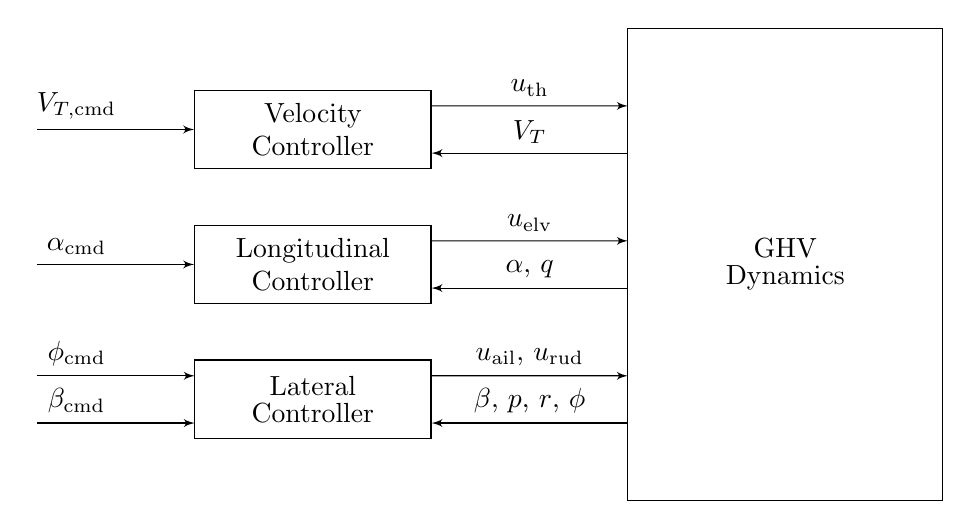
\begin{tikzpicture}[scale=1.0, auto, node distance=2cm,>=latex']
      \matrix[ampersand replacement=\&, row sep=0.7cm, node distance=3.0cm] (regions) at (0,0){%
      \node[block, minimum width=3cm] (R1) {\shortstack{Velocity \\ Controller}}; \\
      \node[block, minimum width=3cm] (R2) {\shortstack{Longitudinal \\ Controller}};\\
      \node[block, minimum width=3cm] (R3) {\shortstack{Lateral \\ Controller}};\\
      };
      \matrix[ampersand replacement=\&, row sep=0.6cm, right of=R1, node distance=4.0cm] (R1out) {%
      \node [coordinate] (R1outx) {};\\
      \node [coordinate] (R1outP) {};\\
      };
      \matrix[ampersand replacement=\&, row sep=0.6cm, right of=R2, node distance=4.0cm] (R2out) {%
      \node [coordinate] (R2outx) {};\\
      \node [coordinate] (R2outP) {};\\
      };
      \matrix[ampersand replacement=\&, row sep=0.6cm, right of=R3, node distance=4.0cm] (R3out) {%
      \node [coordinate] (R3outx) {};\\
      \node [coordinate] (R3outP) {};\\
      };
      \node [coordinate, left of=R1, node distance=3.5cm] (input1) {};
      \node [coordinate, left of=R2, node distance=3.5cm] (input2) {};
      \matrix[ampersand replacement=\&, row sep=0.6cm, left of=R3, node distance=3.5cm] (R3in) {%
      \node [coordinate] (R3inx) {};\\
      \node [coordinate] (R3inP) {};\\
      };
      \node [coordinate, right of=R3inx, node distance=2.0cm] (R3inx2) {};
      \node [coordinate, right of=R3inP, node distance=2.0cm] (R3inP2) {};
      \node [block, right of=R2,node distance=6.0cm, minimum width=4cm, minimum height=6cm] (Q) {\shortstack{GHV \\ Dynamics}};
      %Region 1 outputs
      \draw [->] (R1.east) + (0cm,0.3cm) -- node [pos=0.5]{$u_{\text{th}}$} (R1outx);
      \draw [<-] (R1.east) + (0cm,-0.3cm) -- node [pos=0.5]{$V_{T}$} (R1outP);
      %Region 2 outputs
      \draw [->] (R2.east) + (0cm,0.3cm) -- node [pos=0.5]{$u_{\text{elv}}$} (R2outx);
      \draw [<-] (R2.east) + (0cm,-0.3cm) -- node [pos=0.5]{$\alpha$, $q$} (R2outP);
      %Region 3 outputs
      \draw [->] (R3.east) + (0cm,0.3cm) -- node [pos=0.5]{$u_{\text{ail}}$, $u_{\text{rud}}$} (R3outx);
      \draw [<-] (R3.east) + (0cm,-0.3cm) -- node [pos=0.5]{$\beta$, $p$, $r$, $\phi$} (R3outP);
      %INPUTS
      \draw [->] (input1) -- node [near start]{$V_{T,\text{cmd}}$} (R1);
      \draw [->] (input2) -- node [near start]{$\alpha_{\text{cmd}}$} (R2);
      % Region 3 outputs
      \draw [->] (R3inx) -- node [near start]{$\phi_{\text{cmd}}$} (R3inx2);
      \draw [->] (R3inP) -- node [near start]{$\beta_{\text{cmd}}$} (R3inP2);
    \end{tikzpicture}
    \caption{Inner loop flight control block diagram\label{innercont_block_fig}}
  \end{center}
\end{figure}

In this chapter, the details regarding control strategy that will be used on each of the three control blocks will be presented, as well as some details concerning the individual subsystems themselves.
This includes a baseline control design and analysis, as well as adaptive augmentation for the longitudinal and lateral subsystems.
It is assumed that the state is available for measurement.

\section{Baseline Control Architecture}
The nominal, linear equations of motion describing each of the three subsystems are described by Equation (\ref{eqn:plantxp}) with the addition of the regulated output $z$ as
\begin{equation}
  \label{eqn:xdotp}
  \begin{split}
    \dot{x}_{p}&=A_{p}x_{p}+B_{p}u \\
    z&=C_{zp}x_{p} \\
  \end{split}
\end{equation}
where $x_{p}\in\mathbb{R}^{n_{p}}$, $u\in\mathbb{R}^{m}$, $A_{p}\in\mathbb{R}^{n_{p}\times n_{p}}$, $B_{p}\in\mathbb{R}^{n_{p}\times m}$,$C_{pz}\in\mathbb{R}^{n_{e}\times n_{p}}$, and $z\in\mathbb{R}^{n_{e}}$.
Note again that the dimensions of each of these quantities may differ for each of the three control subsystems.
Each linear plant subsystem is controlled using an LQR-PI full state feedback controller.
The LQR-PI control architecture is most easily represented by augmenting the plant state with an additional integral error state as follows.
Define the integral error state as the difference between a reference command and corresponding regulated output given by
\begin{equation}
  \label{eqn:integralerror}
  \dot{x}_{e}=z_{\text{cmd}}-z
\end{equation}
In this work the regulated outputs happen to all be components of the state vector, but in general this does not have to be the case, and is the motivation for using the general description of the regulated output.
Using the error description in (\ref{eqn:integralerror}), the state vector $x_{p}$ is augmented to include this error by including $x_{e}$ as a state variable
\begin{equation}
  \label{lqrpi_linear_ss_eqn}
  \begin{bmatrix}
    \dot{x}_{p} \\
    \dot{x}_{e}
  \end{bmatrix}
  =
  \begin{bmatrix}
    A_{p} & 0 \\
    -C_{pz} & 0
  \end{bmatrix}
  \begin{bmatrix}
    x_{p} \\
    x_{e}
  \end{bmatrix}
  +
  \begin{bmatrix}
    B_{p} \\
    0
  \end{bmatrix}u
  +
  \begin{bmatrix}
    0 \\
    I
  \end{bmatrix}z_{\text{cmd}}
\end{equation}
Writing the linear state-space representation in Equation~\ref{lqrpi_linear_ss_eqn} more compactly using $x=\bigr[\begin{array}{cc} x_{p}^{\top} & x_{e}^{\top} \end{array}\bigr]^{\top}$ as
\begin{equation}
  \label{lqrpiss}
  \dot{x}=Ax+Bu+B_{\text{ref}}z_{\text{cmd}}
\end{equation}
where $x\in\mathbb{R}^{n}$, $z_{\text{cmd}}\in\mathbb{R}^{n_{e}}$, $A\in\mathbb{R}^{n\times n}$, $B\in\mathbb{R}^{n\times m}$, $B_{\text{ref}}\in\mathbb{R}^{n\times n_{e}}$ and where
\begin{equation}
  A=
  \begin{bmatrix}
    A_{p} & 0 \\
    -C_{pz} & 0
  \end{bmatrix} \quad
  B=
  \begin{bmatrix}
    B_{p} \\
    0
  \end{bmatrix}
  \quad
  B_{\text{ref}}=
  \begin{bmatrix}
    0 \\
    I
  \end{bmatrix}
\end{equation}
The following baseline control law is used
\begin{equation}
  \label{lqrpilaw}
  u_{\text{bl}}=K_{\text{lqr}}^{\top}x
\end{equation}
Substituting the control law (\ref{lqrpilaw}) into (\ref{lqrpiss})
\begin{equation}
  \label{eqn:nomaugmentedss}
  \dot{x}=\left(A+BK_{\text{lqr}}^{\top}\right)x+B_{\text{ref}}z_{\text{cmd}}
\end{equation}
The gain $K_{\text{lqr}}\in\mathbb{R}^{n\times m}$ is selected by minimizing the cost function (\ref{eqn:jcostfunction}), and ensures the closed loop matrix $\left(A+BK_{\text{lqr}}^{\top}\right)$ is Hurwitz.
The matrices $Q_{\text{lqr}}=Q_{\text{lqr}}^{\top}>0$ and $R_{\text{lqr}}=R_{\text{lqr}}^{\top}>0$ are weights which impact the calculation of the feedback gain.
The selection of these matrices and the resulting effect on control performance is discussed in following sections.
\begin{equation}
  \label{eqn:jcostfunction}
  J=\int_{0}^{\infty}\bigr(x(t)^{\top}Q_{\text{lqr}}x(t)+u(t)^{\top}R_{\text{lqr}}u(t)\bigr)dt
\end{equation}
The optimal feedback gain $K_{\text{lqr}}$ for the control law $u=K_{\text{lqr}}^{\top}x$ is then found by solving the following algebraic Riccati equation.
\begin{equation}
  0=A^{\top}P+PA+Q_{\text{lqr}}-PBR_{\text{lqr}}^{-1}B^{\top}P
\end{equation}
where $K_{\text{lqr}}=-(R_{\text{lqr}}^{-1}B^{\top}P)^{\top}$.

\subsubsection*{The Three Control Subsystems}

The three subsystems that the plant was separated into allowed multiple lower order controllers.
Each of the subsystems of the plant for which a controller will be designed is outlined here.

\paragraph{Velocity}
From the sensitivity analysis, the total velocity is decoupled from the rest of the states, allowing a separate controller to be designed to regulate and control only velocity.
The perturbation state and input used in the velocity controller is
\begin{equation}
  \begin{split}
    x_{p,\text{vtot}}&=
    \bigr[
    \begin{array}{c}
      V_{T}
    \end{array}\bigr] \\
    u_{\text{vtot}}&=
    \bigr[
    \begin{array}{c}
      \delta_{\text{th}}
    \end{array}\bigr]
  \end{split}
\end{equation}
For the velocity subsystem $n_{p}=1$ and $m=1$.
Integral action is applied for tracking velocity reference commands.
That is $n_{e}=1$ and $C_{pz}=\bigr[\begin{array}{c}1\end{array}\bigr]$.

\paragraph{Longitudinal}
The longitudinal system as shown through the modal analysis is decoupled from the other subsystems.
In addition to this decoupling, the longitudinal subsystem can be simplified even further by omitting the pitch angle and altitude states.
This is because they are much slower than the pitch rate and angle of attack.
This subsystem has perturbation state vector
\begin{equation}
  \label{long_statevector_eqn}
  \begin{split}
    x_{p,\text{long}}&=
    \bigr[
    \begin{array}{cc}
      \alpha & q
    \end{array}\bigr]^{\top} \\
    u_{\text{long}}&=
    \bigr[
    \begin{array}{c}
      \delta_{\text{elv}}
    \end{array}\bigr]
  \end{split}
\end{equation}
and $n_{p}=2$ and $m=1$.
Integral action is applied for tracking angle of attack reference commands.
That is $n_{e}=1$ and $C_{pz}=\bigr[\begin{array}{cc}1 & 0 \end{array}\bigr]$.

\paragraph{Lateral-Directional States}
The lateral-directional has perturbation state vector
\begin{equation}
  \label{lat_statevector_eqn}
  \begin{split}
    x_{p,\text{latr}}&=
    \bigr[
    \begin{array}{cccc}
      \beta & p & r & \phi
    \end{array}\bigr]^{\top} \\
    u_{\text{latr}}&=
    \bigr[
    \begin{array}{cc}
      \delta_{\text{ail}} & \delta_{\text{rud}}
    \end{array}\bigr]^{\top}
  \end{split}
\end{equation}
and $n_{p}=4$ and $m=2$.
Because there are two independent control inputs, integral action is applied for tracking both angle of sideslip, and roll angle reference commands.
That is $n_{e}=2$ and
\begin{equation}
  C_{pz}=
  \left[
  \begin{array}{cccc}
    1 & 0 & 0 & 0 \\
    0 & 0 & 0 & 1
  \end{array}\right]
\end{equation}

\section{Frequency-Domain Analysis}

Each of the three control subsystems presented above can be represented using the standard servo, or tracking configuration block diagram in Figure~\ref{fig.lqrpiblock}, where $d_{\text{in}}$ is an input load disturbance, $d_{\text{out}}$ is an output load disturbance or sensor bias, and $n$ is sensor noise.
This representation facilitates the following frequency domain analysis of each of the plant and control subsystems, and is different from the conventional representation only by the addition of the reference signal $z_{\text{cmd}}$.
Additionally, with the LQR-PI controller $r=0$.
The frequency domain analysis is done by breaking the loop at various break points, namely at the input to and output from the plant $G(s)$, with the reference command $z_{\text{cmd}}$ set to zero.
At each of these break points the loop transfer function is found and a sinusoidal signal applied at break point input.
The magnitude and phase of the signal when measured at the break point output provides valuable information about the robustness of the control system\ \cite{book.astrommurray.2009}.

\begin{figure}[H]
  \begin{center}
    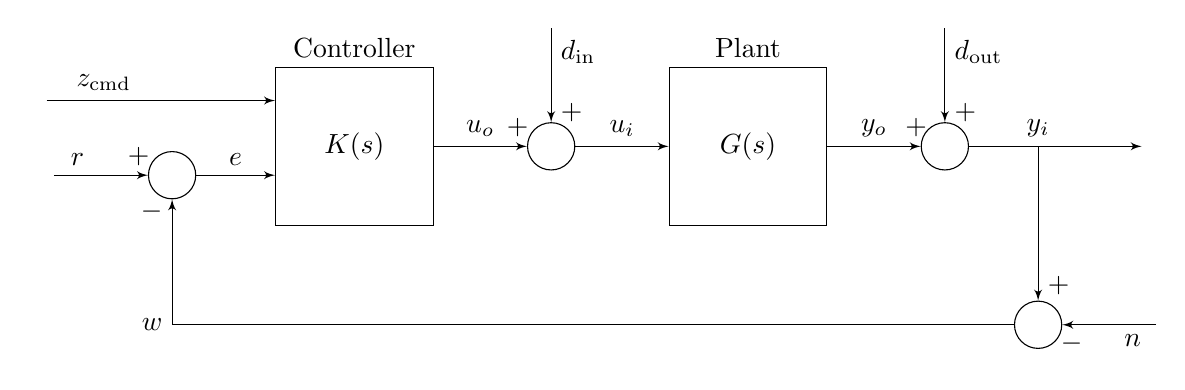
\begin{tikzpicture}[auto, scale=1.0, every node/.style={transform shape}, node distance=1.0cm, >=latex']
      \node[squareblock, minimum height=2cm, minimum width=2cm, label=above:{Controller}] (block1){$K(s)$};
      \node[left=of block1.150, node distance=5.0cm] (j1) {};
      \node[left of=j1, node distance=1.9cm] (input1) {};
      \node[whitesum,left=of block1.200, node distance=1.5cm] (sum1) {};
      \node[input, left of=sum1, node distance=1.5cm](input2){};
      \node[whitesum, right of=block1, node distance=2.5cm] (sum2) {};
      \node[input, above of=sum2,node distance=1.5cm](input3){};
      \node[squareblock, minimum height=2cm, minimum width=2cm, right of=sum2, label=above:{Plant},node distance=2.5cm] (block2) {$G(s)$};
      \node[whitesum, right of=block2,node distance=2.5cm] (sum3) {};
      \node[input, above of=sum3,node distance=1.5cm](input4){};
      \node[output, right of=sum3,node distance=2.5cm] (output1) {};
      \draw[->](sum3) --  node[name=yi,pos=0.4]{$y_{i}$}(output1);
      \node[whitesum, below of=yi,node distance=2.5cm] (sum4) {};
      \node[input, right of=sum4,node distance=1.5cm](input5){};
      \draw[->](input1) -- node[near start]{$z_{\text{cmd}}$} (block1.150);
      \draw[->](input2) -- node[near start]{$r$} node[pos=0.9] {$+$} (sum1);
      \draw[->](sum1) -- node{$e$} (block1.200);
      \draw[->](block1) -- node{$u_{o}$} node[pos=0.9]{$+$} (sum2);
      \draw[->](input3) -- node[near start]{$d_{\text{in}}$} node[pos=0.9] {$+$} (sum2);
      \draw[->](sum2) -- node{$u_{i}$} (block2);
      \draw[->](block2) -- node{$y_{o}$} node[pos=0.95] {$+$} (sum3);
      \draw[->](input4) -- node[near start]{$d_{\text{out}}$} node[pos=0.9] {$+$} (sum3);
      \draw[->](yi) -- node[pos=0.9] {$+$} (sum4);
      \draw[->](input5) -- node[near start]{$n$} node[pos=0.9] {$-$} (sum4);
      \draw[->](sum4) -| node{$w$} node[pos=0.95] {$-$} (sum1);
    \end{tikzpicture}
    \caption{General MIMO feedback control block diagram\label{fig.lqrpiblock}}
  \end{center}
\end{figure}

This frequency domain analysis guides the selection of the weighting matrices in (\ref{eqn:jcostfunction}) which ultimately dictate the corresponding feedback gain.
By completing a frequency domain analysis, the weighting matrices are adjusted until satisfactory level of robustness is achieved.

\subsection{The Different Loop Transfer Functions}

The following give various transfer functions for a plant and controller system represented by Figure~\ref{fig.lqrpiblock}.
The following are titled as transfer functions, but they could actually be transfer matrices.
In the case of SISO systems, multiplication is commutative, but care was taken in the following expressions to consider the MIMO case and preserve pre- and post- multiplication when making algebraic manipulations.
It is also worth noting that many of the other transfer functions between the inputs $r$, $d_{\text{in}}$, $d_{\text{out}}$, and $n$ and the five outputs are described by the transfer functions below, but the transfer functions will be described as relationships between the input and output which is of greatest interest in analyzing the control system.
In the following section $I$ is used to denote the identity matrix, where the size is obvious.

\subsubsection{Input}

\paragraph{Loop Gain Transfer Function}
Breaking the loop at the plant input, the transfer function from $u_{i}$ to $u_{o}$ is given by
\begin{equation}
  L_{u}(s)=K(s)G(s)
\end{equation}

\paragraph{Return Difference Transfer Function}
Differencing the input $u_{i}$ and output $u_{o}$ gives the return difference transfer function
\begin{equation}
  I+L_{u}(s)
\end{equation}

\paragraph{Sensitivity Transfer Function}
The input sensitivity transfer function is from $d_{\text{in}}$ to $u_{i}$ and is given by
\begin{equation}
  S_{u}(s)=\bigr(I+L_{u}(s)\bigr)^{-1}
\end{equation}

\paragraph{Complementary Sensitivity Transfer Function}
Unlike the $T_{y}(s)$, the input complementary sensitivity transfer function does not represent an relationship between any of the system inputs and outputs.
This transfer function is given by using the identity $S_{u}(s)+T_{u}(s)=I$, hence the name complementary sensitivity transfer function, but otherwise there is little intuition regarding what this transfer function represents, and it won't be used in the frequency domain analysis.
\begin{equation}
  T_{u}(s)=L_{u}(s)\bigr(I+L_{u}(s)\bigr)^{-1}
\end{equation}
Note also that $L(I+L)^{-1}=(I+L)^{-1}L$ which can be shown by pre- and post- multiplying both sides by $(I+L)$.

\subsubsection{Output}
\paragraph{Loop Gain Transfer Function}
Evaluate the transfer function from break point input $y_{i}$ to break point output $y_{o}$ while all other signals are zero.
\begin{equation}
  L_{y}(s)=G(s)K(s)
\end{equation}

\paragraph{Return Difference Transfer Function}
Differencing the input $y_{i}$ and output $y_{o}$ gives
\begin{equation}
  I+L_{y}(s)
\end{equation}

\paragraph{Sensitivity Transfer Function}
The output sensitivity is from $d_{\text{out}}$ to $y_{i}$ with all other signals are zero.
\begin{equation}
  S_{y}(s)=\bigr(I+L_{y}(s)\bigr)^{-1}
\end{equation}

\paragraph{Complementary Sensitivity Transfer Function}
Unlike $T_{u}(s)$, this transfer function represents the relationship between the noise $n$ and the output $y_{o}$.
This transfer function also satisfies the identity $S_{y}(s)+T_{y}(s)=I$, hence the name complementary sensitivity transfer function.
\begin{equation}
  T_{y}(s)=L_{y}(s)\bigr(I+L_{y}(s)\bigr)^{-1}
\end{equation}

\subsubsection*{Representation of LQR-PI Controller}

In order to evaluate the loop transfer functions, the LQR-PI controller must be represented as a dynamic compensator, that is, a transfer matrix, as opposed to expressing it as an augmentation to the plant state space description.
Here the LQR-PI controller for the longitudinal subsystem is shown, and the process of expressing the other subsystem controllers this way is the same.
Because the longitudinal subsystem has two states and one input, the controller should be described by a system with three inputs (the reference command, and feedback from each of the two states) and one output.
The input to the controller is $\bigr[\begin{array}{ccc} \alpha_{\text{cmd}} & -\alpha & -q \end{array}\bigr]^{\top}$ and the output is $u$, in this case the commanded elevator deflection angle.
\begin{align}
  \dot{x}_{e}&=
  \begin{bmatrix}
    1 & 1 & 0
  \end{bmatrix}
  \begin{bmatrix}
    \alpha_{\text{cmd}} \\
    -\alpha \\
    -q
  \end{bmatrix} \\
  u&=
  \begin{bmatrix}
    k_{e}
  \end{bmatrix}
  \begin{bmatrix}
    x_{e}
  \end{bmatrix}+
  \begin{bmatrix}
    0 & -k_{\alpha} & -k_{q}
  \end{bmatrix}
  \begin{bmatrix}
    \alpha_{\text{cmd}} \\
    -\alpha \\
    -q
  \end{bmatrix}
\end{align}
The matrices corresponding this state space representation of the controller are the following
\begin{equation}
  A_{c}=0 \quad B_{c}=
  \begin{bmatrix}
    1 & 1 & 0
  \end{bmatrix}
  \quad C_{c}=
  \begin{bmatrix}
    k_{e}
  \end{bmatrix}
  \quad D_{c}=
  \begin{bmatrix}
    0 & -k_{\alpha} & -k_{q}
  \end{bmatrix}
\end{equation}
This state space representation was then converted to a transfer matrix representation for frequency domain analysis.
This transfer matrix was $1\times3$: from the controller input $r$, $-\alpha$, and $-q$ to the output $u_{\text{elv}}$.

\subsubsection*{Multivariable Frequency-Domain Analysis}

The controllers designed in the preceding section can be applied to the nonlinear model and simulated.
The feedback gains may be adjusted, and their performance evaluated using the simulation time response.
Stability can be checked by looking at the location of the closed-loop poles in the complex plane.
Even though the closed-loop system may be stable and respond very well for the nominal case, a lack of robustness could mean slight change in the plant parameters could cause the system to perform very poorly, and even become unstable.

The controller must be designed so the system performs well not only in the nominal case, but also when subject to disturbances such as wind gusts and sensor noise, and uncertainties in the plant parameters.
For SISO classical controllers, frequency domain tools such as the Bode plot are used.
The Bode for a single transfer function is not so easily extended to MIMO systems which is described by transfer function matrices.
Because of this, the singular values of the transfer matrices must be used.

In classical design the loop transfer function needed to be large at low frequency for good command following and disturbance rejection, but small at high frequency for noise attenuation.
When extending to transfer function matrices, a measure of the ``smallness'' of the matrix is needed: the singular values.
The singular value decomposition of a matrix $M$ is given by the factorization
\begin{equation}
  M=U\Sigma V^{*}
\end{equation}
where $(\cdot)^{*}$ denotes the Hermitian, or conjugate transpose, and $U$ and $V^{*}$ are real or complex unitary matrices, i.e. $U^{*}U=UU^{*}=I$, and $\Sigma$ is diagonal matrix with nonnegative real numbers on the diagonal.
The diagonal entries of $\Sigma$ are the singular values of $M$.
Taking the Hermitian transpose of $M$ gives $M^{*}=(U\Sigma V^{*})^{*}=V\Sigma^{*}U^{*}$.
Both pre- and post- multiplying $M$ with its Hermitian transpose:
\begin{equation}
  \begin{split}
    MM^{*}&=U\Sigma V^{*}V\Sigma^{*}U^{*}=U\Sigma \Sigma^{*}U^{*} \\
    M^{*}M&=V\Sigma^{*}U^{*}U\Sigma V^{*}=V\Sigma^{*}\Sigma V^{*}
  \end{split}
\end{equation}
Since $\Sigma$ is diagonal, this can be rearranged into the following eigenvalue problems, allowing the singular values to be found as the non-zero eigenvalues of $M^{*}M$ or $MM^{*}$.
\begin{equation}
  \begin{split}
    (MM^{*})U&=U(\Sigma \Sigma^{*}) \\
    (M^{*}M)V&=V(\Sigma^{*}\Sigma)
  \end{split}
\end{equation}
When the matrix $M$ is a transfer matrix $H(j\omega)$, the magnitude at a any frequency $\omega$ will depend on the direction of the input.
Different singular values will be excited depending on the input.
However, for any input the magnitude of $H(j\omega)$ is bounded above by its maximum singular value $\overline{\sigma}(H(j\omega))$ and below by its minimum singular value $\underline{\sigma}(H(j\omega))$.
To generate the singular value plot for the linear system $\dot{x}=Ax+Bu$ with output given by $y=Cx$, the transfer matrix $H$ must first be calculated:
\begin{equation}
  H(s)=C(sI-A)^{-1}B
\end{equation}
The singular values for each transfer matrix $H$ above can then be plotted versus frequency.
The following equations to determine the gain and phase margin for a MIMO system are found in Reference\ \cite{lavretskywise.book.2013} and presented here for completeness.
First define
\begin{equation}
  \alpha_{\sigma}=\min_{\omega}\underline{\sigma}\bigr(I+L_{u}(s)\bigr)
\end{equation}
\begin{equation}
  \beta_{\sigma}=\min_{\omega}\underline{\sigma}\bigr(I+L_{u}(s)^{-1}\bigr)
\end{equation}
Calculate the phase margin and gain margin from the return difference matrix as
\begin{equation}
  GM_{I+L}=\left[\frac{1}{1+\alpha_{\sigma}},\frac{1}{1-\alpha_{\sigma}}\right]\quad
  PM_{I+L}=\pm2\sin^{-1}\biggr(\frac{\alpha_{\sigma}}{2}\biggr)
\end{equation}
and from the stability robustness matrix as
\begin{equation}
  GM_{I+L^{-1}}=\left[1-\beta_{\sigma},1+\beta_{\sigma}\right]\quad
  PM_{I+L^{-1}}=\pm2\sin^{-1}\biggr(\frac{\beta_{\sigma}}{2}\biggr)
\end{equation}
Taking the union of these two gain and phase margin expressions yield the following multivariable margins.
\begin{equation}
  GM=GM_{I+L}\cup GM_{I+L^{-1}}\quad
  PM=PM_{I+L}\cup PM_{I+L^{-1}}
\end{equation}
These margins are more conservative than classical stability margins calculated for SISO systems.

\subsection{Closing Inner Flight Control Loops}

In this section the selection of the LQR weighting matrices and their impact on the frequency domain properties of the loop transfer functions is discussed.
The weighting matrices for each of the three baseline controllers are given, as well as the baseline feedback control gains that resulted.
Note that the units for the angle measurements used in feedback are radians, while the control surface deflections are in degrees, making many of the gains appear 57.3 times larger than what might be expected.
Note again that the frequency domain plots shown here are for the nominal flight condition.

\subsubsection*{Velocity Controller}

The design of the LQR-PI velocity controller followed the procedure as outlined above.
The values of the components of the LQR weighting matrices are given in Table~\ref{vtot_weights_tab}.
The velocity subsystem is open-loop stable, so the controller only had to provide the capability for reference command tracking.
Additionally, the throttle on aircraft, and hypersonic vehicles in particular, is adjust very slowly.
Because of this, the gains were kept relatively small, keeping the crossover frequency low, and the margins very conservative.

\begin{figure}[H]
  \begin{center}
    \includegraphics[width=4.0in]{\figurepath/results_vtotbode_v1.eps}
     \caption{Velocity loop transfer function Bode plot}
  \end{center}
\end{figure}

\begin{figure}[H]
  \begin{center}
    \includegraphics[width=6.5in]{\figurepath/results_vtotsigma_v1.eps}
     \caption{Velocity loop transfer function singular values}
  \end{center}
\end{figure}

\begin{table}[h]
  \centering
  \caption{Velocity controller LQR weights}
  \small
  \begin{tabular}{ccc}
    \toprule
    & Weight & Value \\
    \midrule
    \multirow{2}{*}{$Q_{\text{lqr}}$} & $V_{T}$ & 0 \\
    & $x_{e}$ & 1 \\
    \midrule
    $R_{\text{lqr}}$ & $u_{\text{th}}$ & 0.03 \\
    \bottomrule
  \end{tabular}\label{vtot_weights_tab}
\end{table}

\begin{equation*}
  {K_{\text{vtot}}}=
  \left[
  \begin{array}{cc}
    0.21 & -0.58
  \end{array}\right]^{\top}
\end{equation*}

\begin{equation*}
  GM=\text{Inf}
  \hspace{0.5in}
  PM=65.6\text{~deg}
\end{equation*}

\subsubsection*{Longitudinal Controller}

Unlike the velocity controller, the longitudinal dynamics of the GHV are highly unstable.
Because of this, the longitudinal control subsystem had to stabilize the plant in addition to providing reference command tracking.

\begin{figure}[H]
  \begin{center}
    \includegraphics[width=4.0in]{\figurepath/results_longbode_v1.eps}
     \caption{Longitudinal loop transfer function Bode plot\label{fig:longbode}}
  \end{center}
\end{figure}

\begin{figure}[H]
  \begin{center}
    \includegraphics[width=6.5in]{\figurepath/results_longsigma_v1.eps}
     \caption{Longitudinal loop transfer function singular values\label{fig:longsigma}}
  \end{center}
\end{figure}

Also unlike the velocity subsystem the longitudinal control system should not be slow, although there is an upper limit on the crossover frequency based on the vehicle and actuator dynamics.
The Bode and singular value plots in Figure~\ref{fig:longbode} and Figure~\ref{fig:longsigma}, respectively, give a graphical representation of the frequency domain properties for this subsystem.

For this subsystem, tolerating a small crossover frequency in allowed a greater level of robustness to be achieved, at the expense of sacrificing the speed of the response.
While slow response characteristics might be acceptable for a large transport aircraft, the GHV must be able to quickly respond to commands in order to execute aggressive maneuvers.
Making the crossover frequency increasingly large eventually has diminishing returns, as due to the dynamics of the vehicle and the actuators, there is a limit on how quickly the vehicle can respond to commands.
Additionally, increasing the crossover frequency deteriorates the margins.
For this reason a crossover frequency of approximately 2 Hz was selected.

\begin{table}[H]
  \centering
  \caption{Longitudinal controller LQR weights}
  \small
  \begin{tabular}{ccc}
    \toprule
    & Weight & Value \\
    \midrule
    \multirow{3}{*}{$Q_{\text{lqr}}$} & $\alpha$ & 0 \\
    & $q$ & 0 \\
    & $x_{e}$ & 170 \\
    \midrule
    $R_{\text{lqr}}$ & $u_{\text{elv}}$ & 0.0001 \\
    \bottomrule
  \end{tabular}\label{long_weights_tab}
\end{table}

\begin{equation*}
  {K_{\text{long}}}=
  \left[
  \begin{array}{ccc}
    -434 & -67.8 & 1304
  \end{array}\right]^{\top}
\end{equation*}

\begin{equation*}
  GM=-14.8\text{~dB}
  \hspace{0.5in}
  PM=71.3\text{~deg}
\end{equation*}

\subsubsection*{Lateral-directional Controller}

The challenges associated with the design of the lateral controller were similar to that of the longitudinal controller in terms of an open loop unstable plant, and requirement for sufficiently large crossover.
The primary difference in the design of the lateral controller was that is multi-output.
This meant Bode plots could not be used, and the singular value plots had to be used.

\begin{figure}[h]
  \begin{center}
    \includegraphics[width=6.5in]{\figurepath/results_latrsigma_v1.eps}
    \caption{Lateral loop transfer matrix singular values\label{fig:latrsigma}}
  \end{center}
\end{figure}

\begin{table}[h]
  \centering
  \caption{Lateral controller LQR weights}
  \small
  \begin{tabular}{ccc}
    \toprule
    & Weight & Value \\
    \midrule
    \multirow{6}{*}{$Q_{\text{lqr}}$} & $\beta$ & 0 \\
    & $p$ & 0 \\
    & $r$ & 0 \\
    & $\phi$ & 10 \\
    & $x_{e,\beta}$ & 10000 \\
    & $x_{e,p}$ & 100 \\
    \midrule
    \multirow{2}{*}{$R_{\text{lqr}}$} & $u_{\text{ail}}$ & 0.02 \\
    & $u_{\text{rud}}$ & 0.02 \\
    \bottomrule
  \end{tabular}\label{latr_weights_tab}
\end{table}

\begin{equation*}
  K_{\text{latr}}=
  \left[
  \begin{array}{rrrrrr}
    435 & -1.86 & -61.8 & -13.7 & -436 & 55.7 \\
    295 & -0.04 & -55.5 & 7.70 & -557 & -43.6
  \end{array}\right]^{\top}
\end{equation*}

\begin{equation*}
  GM=
  \bigr[
  \begin{array}{cc}
    -7.5 & 281.5
  \end{array}\bigr]\text{~dB}
  \hspace{0.5in}
  PM=60.0\text{~deg}
\end{equation*}

\subsubsection*{Inner Loop Controller Summary}

The relevant information describing the three inner loop control subsystems is presented in Table~\ref{tab:crossovers}.
The desired crossover frequencies listed in this table were obtained through recommendations by experts in industry, and reflect values which will provide the desired level of performance while maintaining sufficient robustness.
Additionally, the order of each of the subsystems for which these controllers were designed is summarized in Table~\ref{tab:controlorders}.
All three control subsystems contributed a total of four additional states to the system.
The robustness margins of the three subsystems are summarized in Table~\ref{tab:marginsummary}.

\begin{table}[H]
  \centering
  \caption{Loop transfer function crossover frequencies}
  \small
  \begin{tabular}{lrrr}
    \toprule
    Subsystem & Crossover [rad/s] & Crossover [Hz] & Desired Crossover [Hz]\\
    \midrule
    Velocity & 1.95 & 0.31 & $<1$ \\
    Longitudinal & 16.6 & 2.64 & 2--3 \\
    Lateral & 11.4--17.5 & 1.82--2.78 & 2--3 \\
    \bottomrule
  \end{tabular}\label{tab:crossovers}
\end{table}

\begin{table}[H]
  \centering
  \caption{Subsystem order}
  \small
  \begin{tabular}{lccc}
    \toprule
    Subsystem & Order & Integrators & Augmented Order \\
    \midrule
    Velocity & 1 & $V_{T}$ & 2 \\
    Longitudinal & 2 & $\alpha$ & 3 \\
    Lateral & 4 & $\phi$, $\beta$ & 6 \\
    \bottomrule
  \end{tabular}\label{tab:controlorders}
\end{table}

\begin{table}[H]
  \centering
  \caption{Subsystem robustness margins}
  \small
  \begin{tabular}{lcc}
    \toprule
    Subsystem & Gain Margin [dB] & Phase Margin [deg] \\
    \midrule
    Velocity & \text{Inf} & 65.6 \\
    Longitudinal & -14.8 & 71.3 \\
    Lateral & $\bigr[
    \begin{array}{cc}
      -7.5 & 281.5
    \end{array}\bigr]$ & 43.9 \\
    \bottomrule
  \end{tabular}
  \label{tab:marginsummary}
\end{table}

\subsection{Gain Scheduling}

The previous section described the design of the baseline control gains using a linear model about a nominal trim point.
For maneuvers which depart significantly from this nominal trim condition, the controller performance can deteriorate as the open-loop plant may be very different.
For this reason, it was important to design the feedback gains over a wide range of flight conditions, through gain scheduling.

The primary factor which affects how the open-loop plant behavior changes across the flight envelope is dynamic pressure, and this will be used to schedule the gains.
The dynamic pressure over which the gains will be scheduled is from 800-2000 psf, and is broken into intervals of 100 psf.
In addition to the plant A matrix being different at these different Mach numbers, the weighting matrices $Q_{\text{lqr}}$ and $R_{\text{lqr}}$ used in the cost function can be changed to produce the different gains.
The frequency domain design procedure described in the preceding section could be repeated for each of these 13 dynamic pressure points to carefully select suitable weighting matrices, and corresponding feedback gains.
This would be very time consuming, and instead, the variation of the weighting matrices was also done using dynamic pressure to essentially automate the gain scheduling process.
The idea is that at higher dynamic pressures smaller control deflections are needed to produce the same aerodynamic forces and moments.
So, the nominal input weighting matrix $R_{\text{lqr}}$ was scheduled to be directly proportional to dynamic pressure, thereby penalizing large control inputs more when the dynamic pressure is high and such large control inputs are not necessary.

\begin{figure}[h]
  \begin{center}
    \begin{tikzpicture}[auto, scale=0.8]
      \draw[->] (0,0) -- (14,0) node[anchor=north] {};
      \draw (1,0) node[anchor=north] {800};
      \draw (7,0) node[anchor=north] {\shortstack{Dynamic \\ Pressure [psf]}};
      \draw (0,3.5) node[anchor=south,rotate=90]{\shortstack{Trim \\ Points}};
      \draw (13,0) node[anchor=north] {2000};
      \draw[->] (0,0) -- (0,8) node[anchor=east] {};
      \draw [black] plot [only marks, mark=square*, fill=white!40, minimum height=4.5cm] coordinates {%
      (1,1) (2,1.5) (3,1.8) (4,2.4) (5,2.9) (6,3.5) (7,3.9) (8,4.2) (9,4.7) (10,5.3) (11,5.7) (12,6.2) (13,6.9)
      };
      \draw (1,1) node[anchor=south] {$M=4$};
      \draw (13,6.9) node[anchor=south] {$M=7$};
      \draw (9,3.9) node[anchor=north] {\shortstack{$X_{\text{eq}}$\;,\;$U_{\text{eq}}$ \\ $A_{p}$\;,\;$B_{p}$}};
      \draw (3,6) node[anchor=north] {\shortstack{Different gain $K_{\text{lqr}}$ \\ calculated at each \\ trim point}};
    \end{tikzpicture}
    \caption{Plot of different trim points with dynamic pressure \label{fig:trimpointplot}}
  \end{center}
\end{figure}

The gain schedule was then created off-line, and produced an output containing the trim state and input at each operating point, the corresponding linear model, and the feedback gains.
These data were stored, and the feedback gain is changed by interpolating within the schedule using the slowly varying dynamic pressure measured during flight.
In order to determine the quality of the gain scheduled controller the crossover frequencies and margins were checked at the off-nominal operating points to ensure they were sufficient, and plotted in Figure (\ref{fig:pmgmgs}) and Figure (\ref{fig:pmgmnogs}).

\begin{figure}[H]
  \begin{center}
    \includegraphics[width=5.0in]{\figurepath/pmgmgainschedule.eps}
    \caption{Gain and phase margin of closed-loop subsystems with gain scheduling \label{fig:pmgmgs}}
  \end{center}
\end{figure}

\begin{figure}[H]
  \begin{center}
    \includegraphics[width=5.0in]{\figurepath/pmgmnogainschedule.eps}
    \caption{Gain and phase margin of closed-loop subsystems without gain scheduling \label{fig:pmgmnogs}}
  \end{center}
\end{figure}

These plots show that the nominal fixed gain that was designed about steady level cruise at Mach 6 maintained satisfactory margins across the entire flight envelope, although there was considerable deterioration in the phase margin at lower dynamic pressures, and gain margin for the lateral-directional subsystem especially.
Across the rest of the dynamic pressure range the gain scheduled controller had margins which were about the same as the nominal fixed gain controller, and even had phase margins which were slightly worse at the higher end of the dynamic pressure range.
It is expected that the increased phase margins of the nominal controller over scheduled controller would come at a cost, and might be at the expense of reduced bandwidth.
However, the method used to determine the feedback gains for this gain-scheduled design were not guaranteed to be the best, and with the full ability to tune the LQR weighting matrices at each point a better design could be achieved through more design iterations.
This method only sought to achieve an overall improvement in the margins over the flight envelope, which it did.

\section{Adaptive Control Design}
\label{sec:adaptivedesign}

The baseline controller in the following section has been designed to have adequate gain and phase margins, and thus should be robust to some reasonable variations in plant parameters and other uncertainties.
However, as uncertainties become excessive, as may often occur in hypersonic vehicles during flight, degradation of the baseline controller will be inevitable, and even a robust baseline controller may not be sufficient to ensure stability.
It is for this reason that an adaptive controller was introduced into the picture.

In the presence of parametric uncertainties, it is unknown how the GHV will respond to input commands during flight.
However, under nominal circumstances the plant is completely known and the baseline controller was designed to achieve an ``ideal'' response to a given input, as determined through the design of the LQR-PI controller.
A model-reference adaptive control (MRAC) structure was chosen as it will attempt to recover this nominal behavior by directly using the error between the ideal, or reference model response and actual, or measured vehicle response to drive parameter adaptation.
This adaptive MRAC controller is designed to ensure good command tracking performance and stability in the presence of these uncertainties\ \cite{book.astrom.1989,slotine.appliednonlinear.1991,narendra.stable.2005}.
In addition, the MRAC control architecture can be added without any modification to the baseline controller.
This baseline-plus-adaptive control architecture is represented by the block diagram shown in Figure~\ref{fig.baseplusadaptiveblock}.
It is noted here that the presence in actuator dynamics as shown in this block diagram cause the commanded control input to differ from the applied control.
This fact is not explicitly taken into account in the control design process, hence the use of $u$ to denote both the commanded control output, and the inputs to the plant.
However, the actuator dynamics were implemented in the evaluation model used for generating various simulation studies.
The control system must be robust enough to tolerate, among other things, the presence of these actuator dynamics.

% TODO@dpwiese - replace this with the actual figure used in SM thesis when submitted
\begin{figure}[h]
  \fontsize{10pt}{10pt}\selectfont
  \begin{center}
    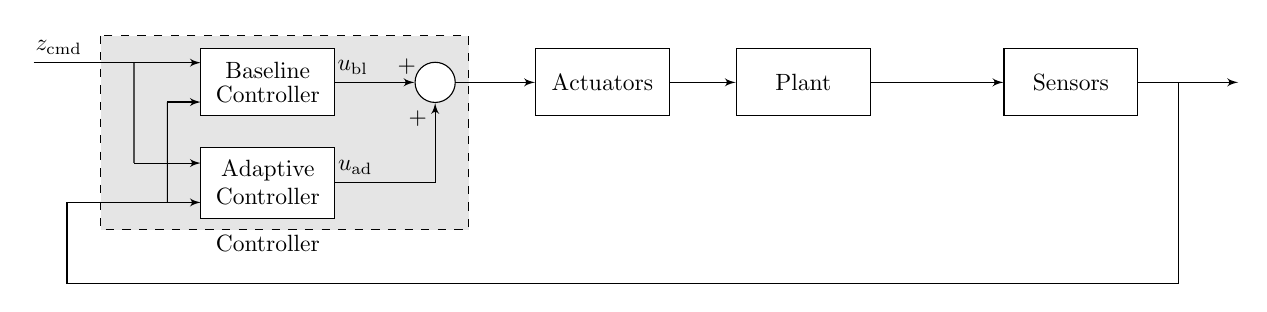
\begin{tikzpicture}[auto, scale=0.85, every node/.style={transform shape}, node distance=1.0cm, >=latex']
      \node[squareblock, minimum height=1cm, minimum width=2cm] (block1){\shortstack[c]{Baseline\\Controller}};
      \node[squareblock, below of=block1, node distance=1.5cm, minimum height=1cm, minimum width=2cm] (block2){\shortstack[c]{Adaptive\\Controller}};
      \matrix[ampersand replacement=\&, row sep=0.5cm, left of=block1,node distance=1cm] (block1in) {%
      \node [coordinate] (b1inA) {};\\
      \node [coordinate] (b1inB) {};\\
      };
      \matrix[ampersand replacement=\&, row sep=0.5cm, left of=block2,node distance=1cm] (block2in) {%
      \node [coordinate] (b2inA) {};\\
      \node [coordinate] (b2inB) {};\\
      };
      \node [left of=b2inB, node distance=0.5cm] (2B) {};
      \node [below of=2B, node distance=0.12cm] (2B2) {};
      \node [left of=b2inA, node distance=1.0cm] (2A) {};
      \node [below of=2A, node distance=0.12cm] (2A2) {};
      \node[whitesum,right of=block1, node distance=2.5cm] (sum1) {};
      \node[squareblock, minimum height=1cm, minimum width=2cm, right of=sum1,node distance=2.5cm] (block3) {Actuators};
      \node[squareblock, minimum height=1cm, minimum width=2cm, right of=block3,node distance=3.0cm] (block4) {Plant};
      \node[squareblock, minimum height=1cm, minimum width=2cm, right of=block4,node distance=4.0cm] (block5) {Sensors};
      \node[output, right of=block5,node distance=2.5cm] (output1) {};
      \node[input, below of=block2,node distance=1.5cm](input2){};
      \draw [->]  (b1inA) + (-2.5cm,0cm) -> node [pos=0.15]{$z_{\text{cmd}}$}  (b1inA);
      \draw [->]  (b1inB) + (-0.5cm,0cm) -> (b1inB);
      \draw [->]  (b2inA) + (-1cm,0cm) -> (b2inA);
      \draw [->]  (b2inB) + (-2.0cm,0cm) -> node[name=TB,node distance=2.5cm]{} (b2inB);
      \draw[->](block5) --  node[name=yi,pos=0.4]{}(output1);
      \draw[-](yi) |- (input2);
      \draw[-](b1inB) + (-0.5cm,0cm) -- (2B2);
      \draw[-](b1inA) + (-1.0cm,0cm) -- (2A2) ;
      \draw[-] (b2inB) + (-2.0cm,0cm) |- (input2);
      \draw[->](block1) -- node[pos=0.22]{$u_{\text{bl}}$} node[pos=0.9]{$+$} (sum1);
      \draw[->](block2) -| node[pos=0.1]{$u_{\text{ad}}$} node[pos=0.9]{$+$} (sum1);
      \draw[->](sum1) -- (block3);
      \draw[->](block3) -- (block4);
      \draw[->](block4) -- (block5);
      \begin{pgfonlayer}{background}
        \path (block1 |- block1)+(-2.5,0.7) node (c) {};
        \path (block2 -| block2)+(3.0,-0.7) node (d) {};
        \path[fill=gray!20, draw, dashed] (c) rectangle (d);
      \end{pgfonlayer}
      \node [below of=block2, node distance = 0.9cm] {Controller};
    \end{tikzpicture}
    \caption{Baseline plus adaptive control block diagram \label{fig.baseplusadaptiveblock}}
  \end{center}
\end{figure}

It was shown in Section~\ref{sec:repofuncertainties} that the nominal plant representation given in Equation (\ref{eqn:plantxp}), when subject to uncertainties, is represented by Equation (\ref{eqn:xdotpunc}) as
\begin{equation}
  \begin{split}
    \dot{x}_{p}&=\bigr(A_{p}+B_{p}\Lambda{W_{p}}^{\top}\bigr)x_{p}+B_{p}\Lambda u \\
    z&=C_{zp}x_{p}
  \end{split}
\end{equation}
This plant model serves as the starting point for the adaptive control design.
In particular, adaptive controllers will be added to the longitudinal and lateral control subsystems, as was shown when introducing the LQR-PI baseline controller in Equation (\ref{lqrpi_linear_ss_eqn}).
Augmenting the uncertain linear plant with an integral error state gives the following
\begin{equation}
  \label{eqn:uncertainss}
  \begin{bmatrix}
    \dot{x}_{p} \\
    \dot{x}_{e}
  \end{bmatrix}=
  \begin{bmatrix}
    A_{p} & 0 \\
    -C_{pz} & 0
  \end{bmatrix}
  \begin{bmatrix}
    x_{p} \\
    x_{e}
  \end{bmatrix}+
  \begin{bmatrix}
    B_{p}\Lambda{W_{p}}^{\top} & 0 \\
    0 & 0
  \end{bmatrix}
  \begin{bmatrix}
    x_{p} \\
    x_{e}
  \end{bmatrix}+
  \begin{bmatrix}
    B_{p} \\
    0
  \end{bmatrix}\Lambda u+
  \begin{bmatrix}
    0 \\
    I
  \end{bmatrix}z_{\text{cmd}}
\end{equation}
Equation (\ref{eqn:uncertainss}) can be expressed using $W^{\top}=[\begin{array}{cc} {W_{p}}^{\top} & 0_{m\times n_{e}} \end{array}]$ as
\begin{equation}
  \begin{bmatrix}
    \dot{x}_{p} \\
    \dot{x}_{e}
  \end{bmatrix}=
  \begin{bmatrix}
    A_{p} & 0 \\
    -C_{pz} & 0
  \end{bmatrix}
  \begin{bmatrix}
    x_{p} \\
    x_{e}
  \end{bmatrix}+
  \begin{bmatrix}
    B_{p} \\
    0
  \end{bmatrix}\Lambda W^{\top}
  \begin{bmatrix}
    x_{p} \\
    x_{e}
  \end{bmatrix}+
  \begin{bmatrix}
    B_{p} \\
    0
  \end{bmatrix}\Lambda u+
  \begin{bmatrix}
    0 \\
    I
  \end{bmatrix}z_{\text{cmd}}
\end{equation}
The integral augmented, uncertain plant for which an adaptive controller will be designed is given by
\begin{equation}
  \label{eqn:uncplant}
  \dot{x}=(A+B\Lambda W^{\top})x+B\Lambda u+B_{\text{ref}}z_{\text{cmd}}
\end{equation}
where $A_{\lambda}=A+B\Lambda W^{\top}$.
This expression reduces to the nominal plant given in Equation (\ref{lqrpiss}) when there is no uncertainty.
The following sections present two model-reference adaptive control strategies.
The first is a classical adaptive controller, and the second is a closed-loop reference model controller.

\subsubsection*{Reference Model}

In order to design a MRAC controller, a suitable reference model is needed.
The reference model defines the desired system performance, with which the plant output is differenced.
It is this difference that is the error signal which drives adaptation.
The classical reference model is given by closing the loop on the nominal plant given by (\ref{eqn:uncplant}) in the absence of uncertainties using the baseline control gain $K_{\text{lqr}}$.
The details concerning the reference model and modifications are provided in the following sections.

\subsection{Classical Model-Reference Adaptive Controller}\label{sec:classicalmrac}

The classical model-reference adaptive controller presented in this section is represented by the block diagram in Figure~\ref{fig:ormblock}.
The approach of adding the adaptive controller on top of the baseline controller is particularly appealing in flight control applications.

\begin{figure}[H]
  \fontsize{10pt}{10pt}\selectfont
  \begin{center}
    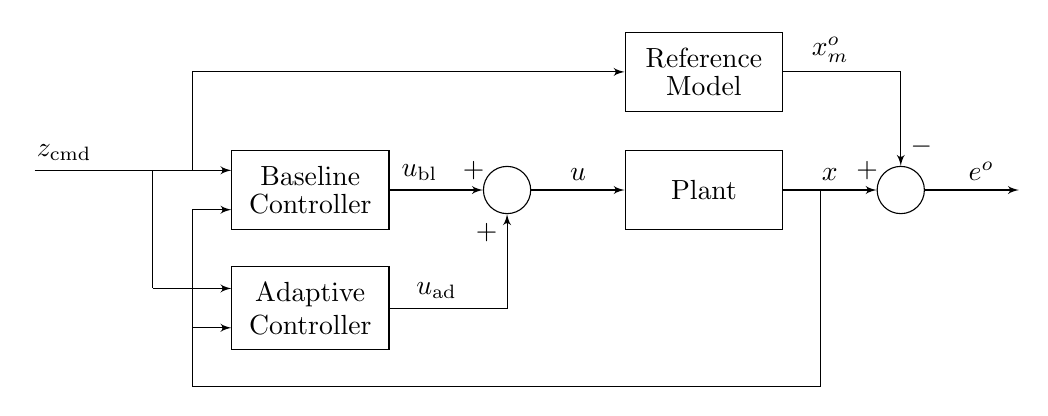
\begin{tikzpicture}[auto, scale=1.0, every node/.style={transform shape}, node distance=1.0cm, >=latex']
      \node[squareblock, minimum height=1cm, minimum width=2cm] (block1){\shortstack[c]{Baseline\\Controller}};
      \node[squareblock, below of=block1, node distance=1.5cm, minimum height=1cm, minimum width=2cm] (block2){\shortstack[c]{Adaptive\\Controller}};
      \matrix[ampersand replacement=\&, row sep=0.5cm, left of=block1,node distance=1cm] (block1in) {%
      \node [coordinate] (b1inA) {};\\
      \node [coordinate] (b1inB) {};\\
      };
      \matrix[ampersand replacement=\&, row sep=0.5cm, left of=block2,node distance=1cm] (block2in) {%
      \node [coordinate] (b2inA) {};\\
      \node [coordinate] (b2inB) {};\\
      };
      \node [left of=b2inB, node distance=0.5cm] (2B) {};
      \node [below of=2B, node distance=0.12cm] (2B2) {};
      \node [left of=b2inA, node distance=1.0cm] (2A) {};
      \node [below of=2A, node distance=0.12cm] (2A2) {};
      \node[whitesum,right of=block1, node distance=2.5cm] (sum1) {};
      \node[squareblock, minimum height=1cm, minimum width=2cm, right of=sum1,node distance=2.5cm] (block3) {Plant};
      \node[squareblock, minimum height=1cm, minimum width=2cm, above of=block3,node distance=1.5cm] (block4) {\shortstack[c]{Reference\\Model}};
      \node[whitesum,right of=block3, node distance=2.5cm] (sum2) {};
      \node[output, right of=sum2,node distance=1.5cm] (output1) {};
      \node[input, below of=block2,node distance=1.0cm](input2){};
      \draw [->]  (b1inA) + (-2.5cm,0cm) -> node [pos=0.15]{$z_{\text{cmd}}$}  (b1inA);
      \draw [->]  (b1inB) + (-0.5cm,0cm) -> (b1inB);
      \draw [->]  (b2inA) + (-1cm,0cm) -> (b2inA);
      \draw [->]  (b2inB) + (-0.5cm,0cm) -> node[name=TB,node distance=2.5cm]{} (b2inB);
      \draw[->](block3) -- node[pos=0.5]{$x$} node[pos=0.9]{$+$} node[name=xi,pos=0.4]{} (sum2);
      \draw[->](sum2) --  node[name=yi,pos=0.4]{} node[pos=0.6]{$e^{o}$} (output1);
      \draw[-](xi) |- (input2);
      \draw[-](b1inB) + (-0.5cm,0cm) -- (2B2);
      \draw[-](b1inA) + (-1.0cm,0cm) -- (2A2) ;
      \draw[-] (b2inB) + (-0.5cm,0cm) |- (input2);
      \draw[->](block1) -- node[pos=0.32]{$u_{\text{bl}}$} node[pos=0.9]{$+$} (sum1);
      \draw[->](block2) -| node[pos=0.2]{$u_{\text{ad}}$} node[pos=0.9]{$+$} (sum1);
      \draw[->](sum1) -- node[pos=0.5]{$u$} (block3);
      \draw[->](block4) -| node[pos=0.2]{$x_{m}^{o}$} node[pos=0.9]{$-$} (sum2);
      \draw [->] (b1inA) + (-0.5cm,0cm) |- (block4);
    \end{tikzpicture}
    \caption{Classical model-reference adaptive control architecture\label{fig:ormblock}}
  \end{center}
\end{figure}

The reference model for this classical model-reference adaptive controller is selected by apply the nominal full state feedback controller $u_{\text{bl}}=K_{\text{lqr}}^{\top}x$ to the nominal plant model, where $K_{\text{lqr}}$ is the baseline control gain gain that was calculated to optimize control of the nominal plant.
That is, using the augmented nominal state and input matrices
\begin{equation*}
  A=
  \begin{bmatrix}
    A_{p} & 0 \\
    -C_{pz} & 0
  \end{bmatrix} \quad
  B=
  \begin{bmatrix}
    B_{p} \\
    0
  \end{bmatrix} \quad
  B_{m}=B_{\text{ref}}
\end{equation*}
with the nominal control gain $K_{\text{lqr}}$, the reference model is given by
\begin{equation}
  \label{eqn:xodotm}
  \dot{x}_{m}^{o}=A_{m}x_{m}^{o}+B_{m}z_{\text{cmd}}
\end{equation}
where $A_{m}=A+BK_{\text{lqr}}^{\top}$ is a Hurwitz matrix.
This reference model will provide the nominal response which will be used in calculating the tracking error which will drive adaptation.
With the reference model given in Eq. (\ref{eqn:xodotm}), the tracking error $e^{o}$ is defined as
\begin{equation}
  \label{eqn:eoerror}
  e^{o}=x-x_{m}^{o}
\end{equation}
The adaptive control law is defined as
\begin{equation}
  \label{eqn:uadporm}
  u_{\text{ad}}=\theta^{\top}x
\end{equation}
where $\theta(t) \in \mathbb{R}^{n\times m}$ is the adaptive parameter.
The following adaptive control gain update law is proposed, where $P^{o}=P^{o\top}>0$, and details on the projection operator are found in references\ \cite{lavretskywise.book.2013,PometPraly.1992} and are summarized in Section~\ref{sec:projection}.
\begin{equation}
  \label{eqn:ormupdatelaw}
  \dot{\tilde{\theta}}=\text{Proj}_{\Gamma}\bigr(\theta,-\Gamma^{o} xe^{o\top}P^{o}B\text{sign}(\Lambda)\bigr)
\end{equation}
The total control is given by summing the nominal and adaptive components giving
\begin{equation}
  \label{eqn:utotal}
  \begin{split}
    u&=u_{\text{bl}}+u_{\text{ad}} \\
    &=(K_{\text{lqr}}+\theta)^{\top}x
  \end{split}
\end{equation}
Substituting the control law (\ref{eqn:utotal}) into Equation (\ref{eqn:uncplant}) the closed-loop system becomes
\begin{equation}
  \dot{x}=\left(A+B\Lambda W^{\top}+B\Lambda(\theta+K_{\text{lqr}})^{\top}\right)x+B_{\text{ref}}z_{\text{cmd}}
\end{equation}
Comparing this expression to the reference model, the existence of an ideal feedback gain matrix $\theta^{*}$ that results in perfect reference model tracking can be verified from the following expression.
\begin{equation}
  \label{eqn:matchingcondition}
  A+B\Lambda W^{\top}+B\Lambda(\theta^{*}+K_{\text{lqr}})^{\top}=A+BK_{\text{lqr}}^{\top}
\end{equation}
The adaptive parameter error is defined as
\begin{equation}
  \tilde{\theta}=\theta-\theta^{*}
\end{equation}
Differentiating Equation (\ref{eqn:eoerror}), and substituting (\ref{eqn:uncplant}) and (\ref{eqn:xodotm}) in, the error dynamics can be expressed as
\begin{equation}
  \dot{e}^{o}=A_{\lambda}x+B\Lambda u+B_{\text{ref}}z_{\text{cmd}}-\bigr(A_{m}x_{m}^{o}+B_{m}z_{\text{cmd}}\bigr)
\end{equation}
Substituting Eq. (\ref{eqn:utotal}), and using $B_{m}=B_{\text{ref}}$ the error dynamics become
\begin{equation}
  \dot{e}^{o}=Ax+B\Lambda W^{\top}x+B\Lambda(\theta+K_{\text{lqr}})^{\top}x+B_{\text{ref}}z_{\text{cmd}}-A_{m}x_{m}^{o}-B_{\text{ref}}z_{\text{cmd}}
\end{equation}
Using $A_{m}=A+BK_{\text{lqr}}^{\top}$ and (\ref{eqn:matchingcondition}) the following expression is obtained
\begin{equation}
  A=A_{m}-B\Lambda W^{\top}-B\Lambda(\theta^{*}+K_{\text{lqr}})^{\top}
\end{equation}
This allows the error dynamics to be written as
\begin{equation}
  \dot{e}^{o}=\left(A_{m}-B\Lambda W^{\top}-B\Lambda(\theta^{*}+K_{\text{lqr}})^{\top}+B\Lambda W^{\top}+B\Lambda(\theta+K_{\text{lqr}})^{\top}\right)x-A_{m}x_{m}^{o}
\end{equation}
which finally simplify to
\begin{equation}
  \label{eqn:eodotfin}
  \dot{e}^{o}=A_{m}e^{o}+B\Lambda{\tilde{\theta}}^{\top}x
\end{equation}

The goal of the adaptive controller is to drive the error $e^{o}(t)$ to zero by adjusting the parameter $\theta(t)$.
The following candidate Lyapunov function is proposed, where $\Gamma^{o}\in\mathbb{R}^{n\times n}$ is a symmetric, invertible, positive definite gain matrix, and the operation $|\cdot|$ takes the absolute value of each entry of the matrix argument.

\begin{equation}
  V(e^{o},\tilde{\theta})=e^{o\top}P^{o}e^{o}+\text{tr}\bigr(\tilde{\theta}^{\top}\Gamma^{o-1}\tilde{\theta}|\Lambda|\bigr)
\end{equation}
Differentiating
\begin{equation}
  \label{eqn:Vodot1}
  \dot{V}={\dot{e}}^{o\top}P^{o}e^{o}+e^{o\top}P^{o}\dot{e}^{o}+
  \text{tr}\bigr(\dot{\tilde{\theta}}^{\top}\Gamma^{o-1}\tilde{\theta}|\Lambda|\bigr)
  +\text{tr}\bigr({\tilde{\theta}}^{\top}\Gamma^{o-1}\dot{\tilde{\theta}}|\Lambda|\bigr)
\end{equation}
Substituting Eq. (\ref{eqn:eodotfin}) into Eq. (\ref{eqn:Vodot1}), and letting $-Q^{o}={A_{m}}^{\top}P^{o}+P^{o}A_{m}$ gives
\begin{equation}
  \label{eqn:Vodot2}
  \dot{V}=-e^{o\top}Q^{o}e^{o}+2x^{\top}{\tilde{\theta}}\Lambda{B_{1}}^{\top}P^{o}e^{o}
  +\text{tr}\bigr(\dot{\tilde{\theta}}^{\top}\Gamma^{o-1}\tilde{\theta}|\Lambda|\bigr)
  +\text{tr}\bigr({\tilde{\theta}}^{\top}\Gamma^{o-1}\dot{\tilde{\theta}}|\Lambda|\bigr) \\
\end{equation}
Substituting (\ref{eqn:ormupdatelaw}) into (\ref{eqn:Vodot2}) and letting $y=-xe^{o\top}P^{o}B_{1}\text{sign}(\Lambda)$ gives
\begin{equation}
  \dot{V}=-e^{o\top}Q^{o}e^{o}
  +2\text{tr}\left(\tilde{\theta}^{\top}\bigr(\Gamma^{o-1}\text{Proj}_{\Gamma}(\theta,-\Gamma^{o}y)-y\bigr)|\Lambda|\right)
\end{equation}
The following property of the projection operator as given in Reference\ \cite{lavretskywise.book.2013}
\begin{equation}
  \tilde{\theta}^{\top}\bigr(\Gamma^{-1}\text{Proj}_{\Gamma}(\theta,\Gamma y)-y\bigr)\leq 0
\end{equation}
implies $\dot{V}(e^{o},\theta)\leq 0$.
Thus, the candidate Lyapunov function which was proposed does serve as a valid Lyapunov function for this system.

\subsection{Closed-Loop Model-Reference Adaptive Controller}\label{sec:crmmrac}

In this section, a modification to the classical model-reference adaptive controller described in Section~\ref{sec:classicalmrac} is introduced.
This modification includes an observer-like gain in the reference model, with feedback from the state $x$.
This is referred to as a closed-loop reference model (CRM), and can provide improved transient properties over the classical model-reference adaptive controller, which we denote as the open-loop reference model (ORM) controller\ \cite{gibson.aiaacrm.2012}.
The modified reference model is given by
\begin{equation}
  \label{eqn:xcdotm}
  \dot{x}_{m}^{c}=A_{m}x_{m}^{c}+B_{m}z_{\text{cmd}}-L(x-x_{m}^{c})
\end{equation}
From Equation (\ref{eqn:xcdotm}) it can be seen that the inclusion of the gain $L$ allows the closed-loop reference model response to deviate from that of the open-loop reference model.
In the case when the gain $L$ is reduced to zero, the open-loop reference model is recovered.
This modification to the classical MRAC structure was chosen in an attempt to not only improve the transient response of the system, but also as a potential to provide other improvements such as increased time delay margin, and greater tolerance of parametric uncertainties.

\begin{figure}[h]
  \fontsize{10pt}{10pt}\selectfont
  \begin{center}
    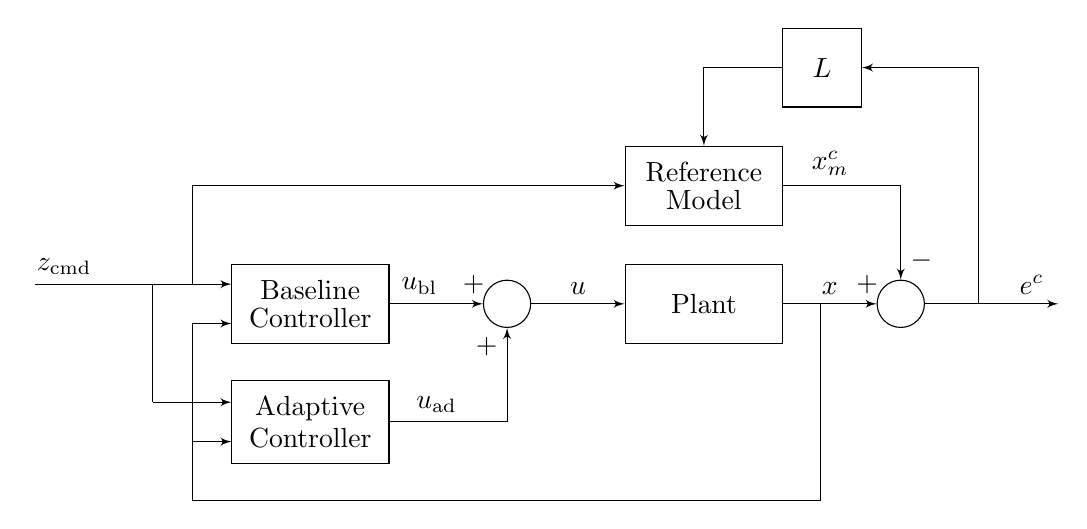
\begin{tikzpicture}[auto, scale=1.0, every node/.style={transform shape}, node distance=1.0cm, >=latex']
      \node[squareblock, minimum height=1cm, minimum width=2cm] (block1){\shortstack[c]{Baseline\\Controller}};
      \node[squareblock, below of=block1, node distance=1.5cm, minimum height=1cm, minimum width=2cm] (block2){\shortstack[c]{Adaptive\\Controller}};
      \matrix[ampersand replacement=\&, row sep=0.5cm, left of=block1,node distance=1cm] (block1in) {%
      \node [coordinate] (b1inA) {};\\
      \node [coordinate] (b1inB) {};\\
      };
      \matrix[ampersand replacement=\&, row sep=0.5cm, left of=block2,node distance=1cm] (block2in) {%
      \node [coordinate] (b2inA) {};\\
      \node [coordinate] (b2inB) {};\\
      };
      \node [left of=b2inB, node distance=0.5cm] (2B) {};
      \node [below of=2B, node distance=0.12cm] (2B2) {};
      \node [left of=b2inA, node distance=1.0cm] (2A) {};
      \node [below of=2A, node distance=0.12cm] (2A2) {};
      \node[whitesum,right of=block1, node distance=2.5cm] (sum1) {};
      \node[squareblock, minimum height=1cm, minimum width=2cm, right of=sum1,node distance=2.5cm] (block3) {Plant};
      \node[squareblock, minimum height=1cm, minimum width=2cm, above of=block3,node distance=1.5cm] (block4) {\shortstack[c]{Reference\\Model}};
      \node [above of=block4, node distance = 1.5cm] (tempnode) {};
      \node[squareblock, minimum height=1cm, minimum width=1cm, right of=tempnode,node distance=1.5cm] (block5) {$L$};
      \node[whitesum,right of=block3, node distance=2.5cm] (sum2) {};
      \node[output, right of=sum2,node distance=2.0cm] (output1) {};
      \node[input, below of=block2,node distance=1.0cm](input2){};
      \draw [->]  (b1inA) + (-2.5cm,0cm) -> node [pos=0.15]{$z_{\text{cmd}}$}  (b1inA);
      \draw [->]  (b1inB) + (-0.5cm,0cm) -> (b1inB);
      \draw [->]  (b2inA) + (-1cm,0cm) -> (b2inA);
      \draw [->]  (b2inB) + (-0.5cm,0cm) -> node[name=TB,node distance=2.5cm]{} (b2inB);
      \draw[->](block3) -- node[pos=0.5]{$x$} node[pos=0.9]{$+$} node[name=xi,pos=0.4]{} (sum2);
      %\draw[->](sum2) --  node[name=yi,pos=0.4]{} node[pos=0.6]{$e^{c}$} (output1);
      \draw[->](sum2) --  node[name=yi,pos=0.4]{} node[pos=0.8]{$e^{c}$} (output1);
      \node [below of=yi, node distance = 0.25cm] (tempnode2) {};
      \draw[-](xi) |- (input2);
      \draw[->](tempnode2) |- (block5);
      \draw[-](b1inB) + (-0.5cm,0cm) -- (2B2);
      \draw[-](b1inA) + (-1.0cm,0cm) -- (2A2) ;
      \draw[-] (b2inB) + (-0.5cm,0cm) |- (input2);
      \draw[->](block1) -- node[pos=0.32]{$u_{\text{bl}}$} node[pos=0.9]{$+$} (sum1);
      \draw[->](block2) -| node[pos=0.2]{$u_{\text{ad}}$} node[pos=0.9]{$+$} (sum1);
      \draw[->](sum1) -- node[pos=0.5]{$u$} (block3);
      \draw[->](block4) -| node[pos=0.2]{$x_{m}^{c}$} node[pos=0.9]{$-$} (sum2);
      \draw [->]  (b1inA) + (-0.5cm,0cm) |- (block4);
      \draw[->](block5) -| (block4);
    \end{tikzpicture}
    \caption{Closed loop reference model adaptive control architecture\label{fig:crmblock}}
  \end{center}
\end{figure}

The modified reference model Jacobian is defined as
\begin{equation}
  \label{eqn:ambar}
  \overline{A}_{m}=A_{m}+L
\end{equation}
and the tracking error is given by
\begin{equation}
  \label{eqn:ecerror}
  e^{c}=x-x_{m}^{c}
\end{equation}
For the CRM adaptive controller, the same adaptive control law as in (\ref{eqn:uadporm}) is used
\begin{equation}
  \label{eqn:uadpcrm}
  u_{\text{ad}}=\theta^{\top}x
\end{equation}
with the following update law
\begin{equation}
  \label{eqn:crmupdatelaw}
  \dot{\tilde{\theta}}=\text{Proj}_{\Gamma}\bigr(\theta,-\Gamma^{c} xe^{c\top}P^{c}B_{1}\text{sign}(\Lambda)\bigr)
\end{equation}
Note that this update law is the same as that in Equation (\ref{eqn:ormupdatelaw}) is used for the ORM adaptive controller, with the exception of the tracking error term $e^{c}$ now being used in the place of $e^{o}$.
The following candidate Lyapunov function is proposed
\begin{equation}
  V(e^{c},\tilde{\theta})=e^{c\top}P^{c}e^{c}+\text{tr}\bigr(\tilde{\theta}^{\top}\Gamma^{-1}\tilde{\theta}|\Lambda|\bigr)
\end{equation}
which has time derivative
\begin{equation}
  \dot{V}=-e^{c\top}Q^{c}e^{c}
  +2\text{tr}\left(\tilde{\theta}^{\top}\bigr(\Gamma^{-1}\text{Proj}_{\Gamma}(\theta,-\Gamma y)-y\bigr)|\Lambda|\right) \\
\end{equation}
As in the ORM case, it can be shown that $\dot{V}(e^{c},\theta)\leq 0$.
Thus, the candidate Lyapunov function which was proposed serves as a valid Lyapunov function for this system.
It can also be shown that $e^{c}\rightarrow e^{o}$ as $t\rightarrow\infty$.

The inclusion of the feedback gain $L$ in the reference model allows the closed-loop reference model response to depart from the open-loop reference model response.
While this can provide improved transient response and other benefits which are observed in simulation, there is also the potential for $L$ to be made sufficiently large so as to deteriorate the time response of the system.
The ideal time response of the system is essentially defined by the open-loop reference model, and the goal is to minimize the tracking error $e^{o}$.
However, in attempting to realize some benefits through the addition of $L$, the closed-loop reference model behavior will be allowed to deviate from the open-loop reference model.
In doing so, while the tracking error $e^{c}$ may be very small, the overall time response of the system may be poor due to large differences between the behavior of the two reference models.
So, while using the error $e^{c}$ to drive adaptation can improve performance, the tracking error $e^{o}$ should still be considered in analyzing performance of the adaptive control system.

\subsection{The Projection Operator}\label{sec:projection}

The projection operator is a means by which the adaptive gain $\theta$ can be bounded.
This is done by specifying a covex function which forms a ball onto which $\dot{\theta}$ is projected.
Consider Figure~\ref{fig:projection}.
The vector $y$ represents $\dot{\theta}$, specified by the update law.
The present value of $\theta$ determines what the projection operator will do, based on where it is in the ball.

\begin{figure}[H]
  \begin{center}
    \psfrag{s}[br][br][1.0]{$\theta^{*}$}
    \psfrag{b}[tc][tc][1.0]{$\theta_{b}$}
    \psfrag{m}[br][br][1.0]{$m=\theta^{*}-\theta_{b}$}
    \psfrag{d}[tc][tc][1.0]{$\nabla f(\theta)$}
    \psfrag{p}[br][br][1.0]{$\text{Proj}(\theta,y)$}
    \psfrag{y}[bc][bc][1.0]{$y$}
    \psfrag{o}[bc][bc][1.0]{$\Omega_{0}$}
    \psfrag{a}[bc][bc][1.0]{$\Omega_{A}$}
    \psfrag{0}[bl][bl][1.0]{$\{\theta|f(\theta)=0\}$}
    \psfrag{1}[bl][bl][1.0]{$\{\theta|f(\theta)=1\}$}
    \includegraphics[width=3.5in]{\figurepath/projection_v1.eps}
    \caption{The projection operator\label{fig:projection}}
  \end{center}
\end{figure}

The outer radius of the ball is given by $\theta_{\text{max}}$ and determines how large $\|\theta\|$ can get, and the annulus region is defined by $\Delta$.
The projection operator is given by

\begin{equation}
  \text{Proj}_{\Gamma}(\theta,\Gamma y)=
  \begin{cases}
    \Gamma y- \Gamma \frac{(\nabla f(\theta))^{\mathsf{T}}\Gamma y \nabla f(\theta) f(\theta)}{(\nabla f(\theta))^{\mathsf{T}}\Gamma \nabla f(\theta)}, & \text{if }f(\theta)>0\wedge y^{\mathsf{T}}\nabla f(\theta)>0 \\
    \Gamma y, & \text{otherwise}
  \end{cases}
\end{equation}

In order to implement the projection operator in an adaptive law, a convex function is which describes the ball onto which $\dot{\theta}$ will be projected is needed.
Typically the convex functions come in the form of a Euclidean norm squared such as the following.
\begin{equation}
  f(\theta)=\frac{\|\theta\|^{2}-{\theta_{0}}^{2}}{2\Delta{\theta_{0}}+\Delta^{2}}
\end{equation}
where $\theta_{0}$ is the inner radius, defined as $\theta_{0}=\theta_{\text{max}}+\Delta$.

\chapter{Simulation Results}

This chapter contains simulation results demonstrating and comparing the capabilities of the baseline and adaptive controllers when applied to the nonlinear evaluation model as depicted in Figure~\ref{fig:simblockdiagram}.
Before presenting the simulation studies showing the response of the vehicle to different commanded trajectories, some additional uncertainties which were used in the simulations are first outlined.

\begin{figure}[h]
  \fontsize{11pt}{11pt}\selectfont
  \begin{center}
    \begin{tikzpicture}[auto, scale=0.75, every node/.style={transform shape}, node distance=1.0cm, >=latex']
      \node[squareblock, minimum height=1cm, minimum width=2cm] (block1){Baseline};
      \node[squareblock, below of=block1, node distance=1.5cm, minimum height=1cm, minimum width=2cm] (block2){Adaptive};
      \matrix[ampersand replacement=\&, row sep=0.5cm, left of=block1,node distance=1cm] (block1in) {%
      \node [coordinate] (b1inA) {};\\
      \node [coordinate] (b1inB) {};\\
      };
      \matrix[ampersand replacement=\&, row sep=0.5cm, left of=block2,node distance=1cm] (block2in) {%
      \node [coordinate] (b2inA) {};\\
      \node [coordinate] (b2inB) {};\\
      };
      \node [left of=b2inB, node distance=0.5cm] (2B) {};
      \node [below of=2B, node distance=0.12cm] (2B2) {};
      \node [left of=b2inA, node distance=1.0cm] (2A) {};
      \node [below of=2A, node distance=0.12cm] (2A2) {};
      %
      \node[whitesum,right of=block1, node distance=2.0cm] (sum1) {};
      \node[squareblock, minimum height=1cm, minimum width=1.0cm, label=below:{delay}, right of=sum1,node distance=1.5cm] (block3) {$\tau$};
      \node[squareblock, minimum height=1cm, minimum width=1.0cm, label=below:{\shortstack[c]{Actuator\\Dynamics}}, right of=block3,node distance=2.5cm, inner sep= 1mm] (block4) {\includegraphics[width=1.6cm]{\figurepath/actuator_image.png}};
      \node [right of=block4,draw=black, anchor=west,node distance=2.0cm, label=below:{\shortstack[c]{Equations of\\Motion}}, minimum width=2cm, inner sep= 0mm] (block5) {\includegraphics[width=4cm]{\figurepath/ghvclouds.pdf}};
      \node[whitesum,right of=block5, node distance=3.0cm] (sum2) {};
      \node[squareblock, minimum height=1cm, minimum width=1.0cm, right of=sum2,node distance=1.5cm] (block6) {ZOH};
      \node[squareblock, minimum height=1cm, minimum width=1.0cm, right of=block6,node distance=1.6cm] (block7) {Filter};
      \node[output, right of=block7,node distance=1.5cm] (output1) {};
      \node[input, below of=block2,node distance=1.0cm](input2){};
      \node[input, above of=sum2,node distance=1.0cm](input3){};
      \draw [->]  (b1inA) + (-2.5cm,0cm) -> node [pos=0.15]{$z_{\text{cmd}}$}  (b1inA);
      \draw [->]  (b1inB) + (-0.5cm,0cm) -> (b1inB);
      \draw [->]  (b2inA) + (-1cm,0cm) -> (b2inA);
      \draw [->]  (b2inB) + (-2.0cm,0cm) -> node[name=TB,node distance=2.5cm]{} (b2inB);
      \draw[->](block7) --  node[name=yi,pos=0.5]{} (output1);
      \draw[-](yi) |- (input2);
      \draw[-](b1inB) + (-0.5cm,0cm) -- (2B2);
      \draw[-](b1inA) + (-1.0cm,0cm) -- (2A2) ;
      \draw[-] (b2inB) + (-2.0cm,0cm) |- (input2);
      \draw[->](block1) -- (sum1);
      \draw[->](block2) -| (sum1);
      \draw[->](sum1) -- (block3);
      \draw[->](block3) -- (block4);
      \draw[->](block4) -- (block5);
      \draw[->](block5) -- (sum2);
      \draw[->](sum2) -- (block6);
      \draw[->](block6) -- node[name=azoh,pos=0.4]{} (block7);
      \draw[->](input3) -- (sum2);
      %
      \begin{pgfonlayer}{background}
        \path (block1 |- block1)+(-2.5,0.7) node (c) {};
        \path (block2 -| block2)+(2.5,-0.7) node (d) {};
        \path[fill=gray!20, draw, dashed] (c) rectangle (d);
      \end{pgfonlayer}
      %
      \begin{pgfonlayer}{background}
        \path (block6 |- block6)+(-0.9,0.7) node (c) {};
        \path (block7 -| block7)+(0.9,-0.7) node (d) {};
        \path[fill=gray!20, draw, dashed] (c) rectangle (d);
      \end{pgfonlayer}
      \node [above of=block1, node distance = 0.9cm] {100 Hz};
      \node [above of=azoh, node distance = 0.8cm] {600 Hz};
      \node [above of=sum2, node distance = 1.2cm] {noise};
    \end{tikzpicture}
    \caption{Simulation block diagram\label{fig:simblockdiagram}}
  \end{center}
\end{figure}

\section{Additional Uncertainties}

\subsubsection*{Sensor Bias/Noise}

Gaussian white noise was injected into the control loop as shown in Figure~\ref{fig:simblockdiagram}.
The variance of the noise used for each of the different sensor types is shown in Table~\ref{tab:noise}.
Each of these signals were passed through the first order navigation filter model, and fed back to the controller.
The filtered and unfiltered signals are shown in Figure~\ref{fig:noise}.
Additionally, sensor bias was added on feedback of the sideslip angle measurement, as is common to occur in inertially derived incidence measurements.

\begin{table}[H]
  \centering
  \caption{Noise variance\label{tab:noise}}
  \small
  \begin{tabular}{llr}
    \toprule
    Sensor type & Units & Variance \\
    \midrule
    Airspeed & [ft/s] & 1 \\
    Incidence & [rad] & 1e-6 \\
    Angular Rate & [rad/s] & 1e-5 \\
    Euler Angles & [rad] & 1e-6 \\
    Altitude & [ft] & 10 \\
    \bottomrule
  \end{tabular}
\end{table}

\begin{figure}[H]
  \begin{center}
    \includegraphics[width=5.0in]{\figurepath/filtervstate.eps}
    \caption{State measurements before and after navigation filter\label{fig:noise}}
  \end{center}
\end{figure}

\subsubsection*{Time Delay}

A input time delay was included in the simulation block diagram.
This time delay was set to zero when generating all of the simulation results shown in task 1 and task 2 below.
To empirically determine the input time delay margin of the different adaptive control strategies this time delay was varied during simulation until stability could not be maintained when flying a given trajectory.
The largest time delay which the system could tolerate while maintaining stability was recorded as the time delay.
However, since the ability of the controller to stabilize the system is dependent on the maneuver performed, these values are useful mostly for comparing the baseline and different adaptive controllers, as opposed to determining an actual delay margin for a given adaptive system.

\section{Results}

This section contains several simulation studies demonstrating the performance of both the baseline, ORM, and CRM adaptive controller in response to some of the uncertainties described above.
Two particular maneuvers are demonstrated below.
Task 1 is an angle of attack doublet command which begins from steady level cruise at Mach 6, followed by a +3 degree angle of attack command for 4 seconds, then -3 degree command for another 4 seconds, and back to steady level cruise.
Task 2 again begins at steady level cruise, and commands an 80 degree roll step.
Four uncertainties are considered for these two tasks:
\begin{enumerate}[label=\Alph*),itemsep=2pt,parsep=2pt,topsep=0pt,partopsep=0pt] % chktex 9 chktex 10
  \item{Control surface effectiveness}
  \item{Longitudinal CG shift}
  \item{Pitching moment coefficient $C_{m_{\alpha}}$}
  \item{Sensor bias on sideslip measurement}
\end{enumerate}
Each response will be denoted by the task number and letter corresponding to the uncertainty which it is subject to.
For example, 1B corresponds to task 1 with uncertainty B.
The components of the state trim vector $X_{\text{eq}}$ are shown in Table~\ref{tab:trimstate}.

\begin{table}[H]
  \centering
  \caption{Components of trim state vector at nominal flight condition of Mach 6}
  \small
  \begin{tabular}{llr}
    \toprule
    State variable & Units & Value \\
    \midrule
    $V_{T}$ & [ft/s] & 5866 \\
    $\alpha$ & [deg] & -0.59 \\
    $q$ & [deg/s] & 0 \\
    $\theta$ & [deg] & -0.59 \\
    $h$ & [ft] & 80,000 \\
    $\beta$ & [deg] & 0 \\
    $p$ & [deg/s] & 0 \\
    $r$ & [deg/s] & 0 \\
    $\phi$ & [deg] & 0 \\
    \bottomrule
  \end{tabular}\label{tab:trimstate}
\end{table}

\subsection{Task 1: Angle of Attack Doublet}

\begin{figure}[H]
  \begin{center}
    \includegraphics[width=5.0in]{\figurepath/select_longres_cef050b.eps}
    \caption{1A:\ 50\% control surface effectiveness on all surfaces}
  \end{center}
\end{figure}

\begin{figure}[H]
  \begin{center}
    \includegraphics[width=5.0in]{\figurepath/select_longres_cgx090b.eps}
    \caption{1B:\ Longitudinal CG shift: -0.9 ft rearward}
  \end{center}
\end{figure}

\begin{figure}[H]
  \begin{center}
    \includegraphics[width=5.0in]{\figurepath/select_longres_cma400b.eps}
    \caption{1C:\ Pitching moment coefficient $C_{m_{\alpha}}$ scaled $4\times$}
  \end{center}
\end{figure}

\begin{figure}[H]
  \begin{center}
    \includegraphics[width=4.9in]{\figurepath/select_longres_bia016b.eps}
    \caption{1D:\ Sensor bias of $+1.6$ degrees on sideslip measurement}
  \end{center}
\end{figure}

\subsection{Task 2: Roll Step}

\begin{figure}[H]
  \begin{center}
    \includegraphics[width=4.9in]{\figurepath/select_latrres_cef050b.eps}
    \caption{2A:\ 50\% control surface effectiveness on all surfaces}
  \end{center}
\end{figure}

\begin{figure}[H]
  \begin{center}
    \includegraphics[width=4.9in]{\figurepath/select_latrres_cgx160b.eps}
    \caption{2B:\ Longitudinal CG shift: -1.6 ft rearward}
  \end{center}
\end{figure}

\begin{figure}[H]
  \begin{center}
    \includegraphics[width=5.0in]{\figurepath/select_latrres_cma400b.eps}
    \caption{2C:\ Pitching moment coefficient $C_{m_{\alpha}}$ scaled $4\times$}
  \end{center}
\end{figure}

\begin{figure}[H]
  \begin{center}
    \includegraphics[width=5.0in]{\figurepath/select_latrres_bia016b.eps}
    \caption{2D:\ Sensor bias of $+1.6$ degrees on sideslip measurement}
  \end{center}
\end{figure}

In many of the cases presented here, the baseline controller is not able to maintain stability for the given task when subject to uncertainty.
Moreover, the ORM adaptive controller also is not able to maintain stability responses 1B and 1C, whereas the CRM adaptive controller is able to maintain stability.
For task 1, the CRM adaptive controller provides good closed-loop performance, with good transient response, minimal overshoot, almost no oscillations.
In response 1A, the baseline and ORM adaptive controller oscillate slightly more in the time response.
This behavior is even more pronounced as control effectiveness is reduced further, to the point where there is insufficient control authority to maintain stability.
In response 1B, the baseline and ORM adaptive controllers fail to maintain stability.
This is triggered by an oscillation in the lateral-directional dynamics, as can be seen in the full state plots in Appendix A.
However, the CRM adaptive controller maintains stability and good time response performance.
A similar situation is observed in response 1C, as the increased pitching moment coefficient has a very similar influence on the plant dynamics as a rearward CG shift.
In response 1D, the baseline controller becomes unstable very quickly, and both ORM and CRM adaptive controllers perform very well.

Response 2A shows the baseline controller again exhibiting significant oscillations in the time response when control effectiveness is reduced.
Both adaptive controllers significantly reduce this oscillation.
Minimal benefit of the adaptive controllers is observed in responses 2B and 2C, but this is largely due to the limited affect the longitudinal CG shift and pitching moment coefficient have on the lateral directional dynamics which are excited during the roll command.
Finally, response 1D again shows the baseline controller failing to maintain stability when subject to the sensor bias on the sideslip angle measurement.

\subsection{Time Delay Margins}

For some of the tasks and uncertainties demonstrated in simulation above, time delay margins were computed empirically for the three controllers by determining the maximum allowable input time delay that could be tolerated while maintaining stability.
Table~\ref{tab:delaymargins} shows the delay margins for each simulation result presented above.

\begin{table}[H]
  \centering
  \caption{Delay margins for selected responses in milliseconds\label{tab:delaymargins}}
  \small
  \begin{tabular}{lrrr}
    \toprule
    &\multicolumn{3}{c}{Controller} \\
    Response & Baseline & ORM & CRM \\
    \midrule
    1A & 33 & 36 & 41 \\
    1B & n/a & 3 & 18 \\
    1C & 26 & 19 & 19 \\
    2A & 34 & 13 & 26 \\
    \bottomrule
  \end{tabular}
\end{table}

While in the case of 1C and 2A, adaptation reduces the delay margin, all four cases show that the closed-loop reference model controller has a delay margin which is equal to or greater than the comparable open-loop reference model controller.
The delay margin of the CRM controller is at least 73\% that of the baseline controller, while the ORM controller has a delay margin which is as little as 38\% of that for the baseline controller.
Adaptation is required to maintain stability and provide good tracking performance, but must do so without sacrificing the delay margin to an unacceptable level.
The CRM adaptive controller is able to satisfy these requirements better than both the baseline and ORM adaptive controller.

\section{Summary}

In the simulation results presented above, the efficacy of the CRM adaptive controller was demonstrated on the GHV when performing two tasks while subject to four different uncertainties.
These uncertainties included decrease in control effectiveness, center-of-gravity shift, unknown pitching moment coefficient, and sensor bias on sideslip angle measurement.
In half of these cases, the baseline control design was not able to maintain stability, and in two cases the ORM adaptive controller failed.
The CRM adaptive controller maintained stability in all cases.
In addition, considering the cases where stable performance was maintained by the baseline and ORM adaptive controllers, the CRM adaptive showed improved time response behavior.
Finally, when a time delay was introduced at the control input, the CRM adaptive controller maintained a greater percentage of the time-delay margin provided by the baseline controller than the ORM adaptive controller did.
Overall, the CRM adaptive controller offers the best performance, tolerating a reduced control effectiveness of 50\%, rearward center of gravity shift of -0.9 to -1.6 feet (6--11\% of vehicle length), aerodynamic coefficient uncertainty scaled $4\times$ the nominal value, and sensor bias of $+1.6$ degrees on sideslip angle measurement.
The closed-loop reference model adaptive controller maintains at least 73\% of the delay margin provided by the robust baseline design, tolerating input time delays of between 18--46 ms during 3 degree angle of attack doublet, and 80 degree roll step commands.
These results demonstrate the necessity of an adaptive controller to provide stable and acceptable tracking performance, while still maintaining much of the delay margin provided by the robust baseline design.

\chapter{Conclusions and Future Work}

The performance of a generic hypersonic vehicle was evaluated during angle of attack and roll commands, when subject to a loss of control effectiveness, stability derivative uncertainties, and CG shifts, while in the presence of sensor noise, and input delay.
Three controllers were considered: a baseline full-state feedback LQR-PI, and the same baseline controller augmented with a classical open-loop reference model adaptive controller, as well as a closed-loop reference model adaptive controller.
Both  adaptive controllers exhibited improved performance and stability over the baseline controller when given a commanded trajectory in the presence of parametric uncertainties.
In addition, the CRM adaptive controller offered improved delay margin over the ORM adaptive controller.
This adaptive augmented gain-scheduled baseline control architecture maintained stable flight given certain uncertainties when the baseline control alone could not.

\section{Control Performance During Unstart}\label{sec:unstart}

The problem of engine unstart was mentioned above as causing abrupt changes in the vehicle dynamics due to the spillage of the shock train out of the engine inlet.
While the adaptive controller is able to use online information to adjust control parameters to ensure stability given certain plant uncertainties, it is difficult for adaptation to occur quickly enough to react to the changes experienced when unstart occurs.
Future work will examine the performance of the baseline and adaptive controllers during unstart using a simple model discussed briefly below.
Other approaches will attempt to avoid unstart altogether by using state limiters\ \cite{muse.constraints.2011,lavretsky.statelimiting.2010}.

\subsection{Unstart Model}\label{sec:unstartmodel}

A simple qualitative unstart model is developed that incorporates a hard switch which abruptly changes the vehicle dynamics from the started to un-started condition.
This model assumes unstart is a function only of angle of attack, sideslip angle, and Mach number, so as to essentially capture the relationship between mass-capture at the inlet, and unstart\ \cite{bolender.modelling.2009}.
The region of started operation is defined in the $\alpha-\beta-M$ space using ellipses in the $\alpha-\beta$ plane as shown in Figure~\ref{fig:unstartcone}.
When the plant state is such that GHV is operating within the interior of this conical region, the engine remains started.
Operation outside this region triggers unstart.

\begin{figure}[H]
  \begin{center}
    \includegraphics[width=4.0in]{\figurepath/unstart_cone_v2.eps}
    \caption{Ellipses defining region of started engine operation\label{fig:unstartcone}}
  \end{center}
\end{figure}

When unstart occurs the vehicle pitching moment is changed by a constant $\Delta C_{m_{0}}$, and slope $\Delta C_{m_{\alpha}}$ and the yawing moment by $\Delta C_{n_{0}}$, and slope $\Delta C_{n_{\beta}}$.

\begin{equation}
  C_{m}=C_{m_{\text{nom}}}+\Delta C_{m_{0}}+\Delta C_{m_{\alpha}}\alpha
\end{equation}
\begin{equation}
  C_{n}=C_{n_{\text{nom}}}+\Delta C_{n_{0}}+\Delta C_{n_{\beta}}\beta
\end{equation}

All engine force and moment contributions become zero, lift decreases by 20\%, and drag increases by 20\%.
Due to the time scale associated with the engine dynamics, engine unstart will essentially result in an instantaneous change in the plant dynamics.
The numerical values corresponding to the moment coefficient perturbations are examined more closely in Section~\ref{sec:unstartmodel}.
For the purposes of control design, it is assumed that pressure measurements at the combustor and inlet can be used to determine when unstart occurs\ \cite{wang.risk.2012}.

\begin{figure}[H]
  \fontsize{10pt}{10pt}\selectfont
  \begin{center}
    \psfrag{cont}[mc][mc][1.0]{\shortstack[c]{Baseline\\Controller}}
    \psfrag{adp}[mc][mc][1.0]{\shortstack[c]{Adaptive\\Controller}}
    \psfrag{unc}[tc][tc][1.0]{\fontsize{10pt}{10pt}\selectfont\bf\shortstack[c]{Unstart \\ model}}
    \psfrag{plant}[mc][mc][1.0]{Plant}
    \psfrag{r}[bc][bc][1.0]{$z_{\text{cmd}}$}
    \psfrag{un}[bc][bc][1.0]{$u_{\text{bl}}$}
    \psfrag{ua}[bc][bc][1.0]{$u_{\text{ad}}$}
    \psfrag{u}[bc][bc][1.0]{$u$}
    \psfrag{x}[bc][bc][1.0]{$x$}
    \psfrag{s}[mc][mc][1.0]{$+$}
    \includegraphics[width=5.5in]{\figurepath/long_term_goals_block.eps}
    \caption{Closed loop system block diagram with unstart model}
  \end{center}
\end{figure}

As future efforts improve the understanding of unstart, this information will be used to build a better unstart model, and guide the development of new novel adaptive strategies to cope with unstart.

\appendix
\chapter{Figures}

\vspace{4in}
\;

\begin{figure}[H]
  \begin{center}
    \includegraphics[width=6.5in]{\figurepath/state_longres_cef050b.eps}
    \caption{1A:\ State response for reduced control surface effectiveness: 50\% on all surfaces}
  \end{center}
\end{figure}

\begin{figure}[H]
  \begin{center}
    \includegraphics[width=6.5in]{\figurepath/input_longres_cef050b.eps}
    \caption{1A:\ Input response for reduced control surface effectiveness: 50\% on all surfaces}
  \end{center}
\end{figure}

\begin{figure}[H]
  \begin{center}
    \includegraphics[width=6.5in]{\figurepath/state_longres_cgx090b.eps}
    \caption{1B:\ State response for longitudinal CG shift: -0.9 ft rearward}
  \end{center}
\end{figure}

\begin{figure}[H]
  \begin{center}
    \includegraphics[width=6.5in]{\figurepath/input_longres_cgx090b.eps}
    \caption{1B:\ Input response for longitudinal CG shift: -0.9 ft rearward}
  \end{center}
\end{figure}

\begin{figure}[H]
  \begin{center}
    \includegraphics[width=6.5in]{\figurepath/state_longres_cma400b.eps}
    \caption{1C:\ State response for pitching moment coefficient scaled $4\times$}
  \end{center}
\end{figure}

\begin{figure}[H]
  \begin{center}
    \includegraphics[width=6.5in]{\figurepath/input_longres_cma400b.eps}
    \caption{1C:\ Input response for pitching moment coefficient scaled $4\times$}
  \end{center}
\end{figure}

\begin{figure}[H]
  \begin{center}
    \includegraphics[width=6.5in]{\figurepath/state_longres_bia016b.eps}
    \caption{1D:\ State response for sensor bias of $+1.6$ degrees on sideslip measurement}
  \end{center}
\end{figure}

\begin{figure}[H]
  \begin{center}
    \includegraphics[width=6.5in]{\figurepath/input_longres_bia016.eps}
    \caption{1D:\ State response for sensor bias of $+1.6$ degrees on sideslip measurement}
  \end{center}
\end{figure}

\begin{figure}[H]
  \begin{center}
    \includegraphics[width=6.5in]{\figurepath/state_latrres_cef050b.eps}
    \caption{2A:\ State response with 50\% control surface effectiveness on all surfaces}
  \end{center}
\end{figure}

\begin{figure}[H]
  \begin{center}
    \includegraphics[width=6.5in]{\figurepath/input_latrres_cef050b.eps}
    \caption{2A:\ Input response with 50\% control surface effectiveness on all surfaces}
  \end{center}
\end{figure}

\begin{figure}[H]
  \begin{center}
    \includegraphics[width=6.5in]{\figurepath/state_latrres_cgx160b.eps}
    \caption{2B:\ State response with longitudinal CG shift: -1.6 ft rearward}
  \end{center}
\end{figure}

\begin{figure}[H]
  \begin{center}
    \includegraphics[width=6.5in]{\figurepath/input_latrres_cgx160b.eps}
    \caption{2B:\ State response with longitudinal CG shift: -1.6 ft rearward}
  \end{center}
\end{figure}

\begin{figure}[H]
  \begin{center}
    \includegraphics[width=6.5in]{\figurepath/state_latrres_cma400b.eps}
    \caption{2C:\ State response for pitching moment coefficient scaled $4\times$}
  \end{center}
\end{figure}

\begin{figure}[H]
  \begin{center}
    \includegraphics[width=6.5in]{\figurepath/input_latrres_cma400b.eps}
    \caption{2C:\ Input response for pitching moment coefficient scaled $4\times$}
  \end{center}
\end{figure}

\begin{figure}[H]
  \begin{center}
    \includegraphics[width=6.5in]{\figurepath/state_latrres_bia016b.eps}
    \caption{2D:\ State response for sensor bias of $+1.6$ degrees on sideslip measurement}
  \end{center}
\end{figure}

\begin{figure}[H]
  \begin{center}
    \includegraphics[width=6.5in]{\figurepath/input_latrres_bia016b.eps}
    \caption{2D:\ Input response for sensor bias of $+1.6$ degrees on sideslip measurement}
  \end{center}
\end{figure}

\begin{singlespace}
  \bibliography{../bib/thesis-sm}
  \bibliographystyle{plain}
\end{singlespace}

\end{document}
